%%%%%%%%%%%%%%%%%%%%%%%%%%%%%%%%%%%%%%%%%%%%%%%%%%%%%%%%%%%%%%%%%%%%%%%%
%% Customizações do abnTeX2 (http://abnTeX2.googlecode.com)           %%
%% para a Universidade de Fortaleza						              %%
%%                                                                    %%
%% This work may be distributed and/or modified under the             %%
%% conditions of the LaTeX Project Public License, either version 1.3 %%
%% of this license or (at your option) any later version.             %%
%% The latest version of this license is in                           %%
%%   http://www.latex-project.org/lppl.txt                            %%
%% and version 1.3 or later is part of all distributions of LaTeX     %%
%% version 2005/12/01 or later.                                       %%
%%                                                                    %%
%% This work has the LPPL maintenance status `maintained'.            %%
%%                                                                    %%
%% The Current Maintainer of this work is Bruno Lopes                 %%
%%                                                                    %%
%% Project available on: https://github.com/bruno-unifor/unifortex2   %%
%%                                                                    %%
%% Further information about abnTeX2                                  %%
%% are available on http://abntex2.googlecode.com/                    %%
%%                                                                    %%
%%%%%%%%%%%%%%%%%%%%%%%%%%%%%%%%%%%%%%%%%%%%%%%%%%%%%%%%%%%%%%%%%%%%%%%%

%%%%%%%%%%%%%%%%%%%%%%%%%%%%%%%%%%%%%%%%%%%%%%%%%%%%%%%%%%%%%%%%%%%%%%%%
%% Customizações do abnTeX2 (http://abnTeX2.googlecode.com)           %%
%% para a Universidade de Fortaleza						              %%
%%                                                                    %%
%% This work may be distributed and/or modified under the             %%
%% conditions of the LaTeX Project Public License, either version 1.3 %%
%% of this license or (at your option) any later version.             %%
%% The latest version of this license is in                           %%
%%   http://www.latex-project.org/lppl.txt                            %%
%% and version 1.3 or later is part of all distributions of LaTeX     %%
%% version 2005/12/01 or later.                                       %%
%%                                                                    %%
%% This work has the LPPL maintenance status `maintained'.            %%
%%                                                                    %%
%% The Current Maintainer of this work is Bruno Lopes                 %%
%%                                                                    %%
%% Project available on: https://github.com/bruno-unifor/unifortex2   %%
%%                                                                    %%
%% Further information about abnTeX2                                  %%
%% are available on http://abntex2.googlecode.com/                    %%
%%                                                                    %%
%%%%%%%%%%%%%%%%%%%%%%%%%%%%%%%%%%%%%%%%%%%%%%%%%%%%%%%%%%%%%%%%%%%%%%%%

\documentclass[
    a4paper,          % Tamanho da folha A4
    12pt,             % Tamanho da fonte 12pt
    chapter=TITLE,    % Todos os capitulos devem ter caixa alta
    section=TITLE,    % Todas as secoes devem ter caixa alta
    oneside,          % Usada para impressao em apenas uma face do papel
    english,          % Hifenizacoes em ingles
    spanish,          % Hifenizacoes em espanhol
    brazil            % Ultimo idioma eh o idioma padrao do documento
]{abntex2}

% Importações de pacotes
\usepackage[brazil]{babel} 
\usepackage[utf8]{inputenc}                         % Acentuação direta
\usepackage[T1]{fontenc}                            % Codificação da fonte em 8 bits
\usepackage{graphicx}                               % Inserir figuras
\usepackage{amsfonts, amssymb, amsmath}             % Fonte e símbolos matemáticos
\usepackage{booktabs}                               % Comandos para tabelas
\usepackage{verbatim}                               % Texto é interpretado como escrito no documento
\usepackage{multirow, array}                        % Múltiplas linhas e colunas em tabelas
\usepackage{indentfirst}                            % Endenta o primeiro parágrafo de cada seção.
\usepackage{listings}                               % Utilizar codigo fonte no documento
\usepackage{xcolor}
\usepackage{microtype}                              % Para melhorias de justificação?
\usepackage[portuguese,ruled,lined]{algorithm2e}    % Escrever algoritmos
\usepackage{algorithmic}                            % Criar Algoritmos
%\usepackage{float}                                  % Utilizado para criação de floats
\usepackage{amsgen}
\usepackage{lipsum}                                 % Usar a simulação de texto Lorem Ipsum
%\usepackage{titlesec}                               % Permite alterar os títulos do documento
\usepackage{tocloft}                                % Permite alterar a formatação do Sumário
\usepackage{etoolbox}                               % Usado para alterar a fonte da Section no Sumário
\usepackage[nogroupskip,nonumberlist,acronym]{glossaries}                % Permite fazer o glossario
\usepackage{caption}                                % Altera o comportamento da tag caption
\usepackage[alf, abnt-emphasize=bf, bibjustif, recuo=0cm, abnt-etal-cite=3, abnt-etal-list=0,abnt-etal-text=it]{abntex2cite}  % Citações padrão ABNT
%\usepackage[bottom]{footmisc}                      % Mantém as notas de rodapé sempre na mesma posição
%\usepackage{times}                                 % Usa a fonte Times
\usepackage{mathptmx}                               % Usa a fonte Times New Roman
\usepackage{subcaption}
%\usepackage{lmodern}                               % Usa a fonte Latin Modern
%\usepackage{subfig}                                % Posicionamento de figuras
%\usepackage{scalefnt}                              % Permite redimensionar tamanho da fonte
%\usepackage{color, colortbl}                       % Comandos de cores
%\usepackage{lscape}                                % Permite páginas em modo "paisagem"
%\usepackage{ae, aecompl}                           % Fontes de alta qualidade
%\usepackage{picinpar}                              % Dispor imagens em parágrafos
%\usepackage{latexsym}                              % Símbolos matemáticos
%\usepackage{upgreek}                               % Fonte letras gregas
\usepackage{appendix}                               % Gerar o apendice no final do documento
\usepackage{paracol}                                % Criar paragrafos sem identacao
\usepackage{lib/unifortex2}		                    % Biblioteca com as normas da Unifor para trabalhos academicos
\usepackage{pdfpages}                               % Incluir pdf no documento
\usepackage{amsmath}                                % Usar equacoes matematicas

% Organiza e gera a lista de abreviaturas, simbolos e glossario
\makeglossaries

% Gera o Indice do documento
\makeindex


%%%%%%%%%%%%%%%%%%%%%%%%%%%%%%%%%%%%%%%%%%%%%%%%%%%%%
%%          Configuracoes do uniforTeX2            %%
%%%%%%%%%%%%%%%%%%%%%%%%%%%%%%%%%%%%%%%%%%%%%%%%%%%%%

% Opcoes disponiveis

\trabalhoacademico{tccgraduacao}
%\trabalhoacademico{tccespecializacao}
%\trabalhoacademico{dissertacao}
%\trabalhoacademico{tese}

% Define se o trabalho eh uma qualificacao
% Coloque 'nao' para versao final do trabalho

%\ehqualificacao{nao}

% Remove as bordas vermelhas e verdes do PDF gerado
% Coloque 'sim' pare remover

\removerbordasdohyperlink{sim}

% Adiciona a cor Azul a todos os hyperlinks

\cordohyperlink{nao}

%%%%%%%%%%%%%%%%%%%%%%%%%%%%%%%%%%%%%%%%%%%%%%%%%%%%%
%%          Informação sobre a IES                 %%
%%%%%%%%%%%%%%%%%%%%%%%%%%%%%%%%%%%%%%%%%%%%%%%%%%%%%

\ies{Universidade de Fortaleza}
\iessigla{UNIFOR}
\centro{Centro de Ciências Tecnológicas}

%%%%%%%%%%%%%%%%%%%%%%%%%%%%%%%%%%%%%%%%%%%%%%%%%%%%%
%%        Informação para TCC de Graduacao         %%
%%%%%%%%%%%%%%%%%%%%%%%%%%%%%%%%%%%%%%%%%%%%%%%%%%%%%

\graduacaoem{Engenharia de Computação}
\habilitacao{bacharel} % Pode colocar tambem 'licenciada'

%%%%%%%%%%%%%%%%%%%%%%%%%%%%%%%%%%%%%%%%%%%%%%%%%%%%%
%%     Informação para TCC de Especializacao       %%
%%%%%%%%%%%%%%%%%%%%%%%%%%%%%%%%%%%%%%%%%%%%%%%%%%%%%

\especializacaoem{Alfabetização de Crianças}

%%%%%%%%%%%%%%%%%%%%%%%%%%%%%%%%%%%%%%%%%%%%%%%%%%%%%
%%         Informação para Dissertacao             %%
%%%%%%%%%%%%%%%%%%%%%%%%%%%%%%%%%%%%%%%%%%%%%%%%%%%%%

\programamestrado{Programa de Pós-Graduação em Informática Aplicada}
\nomedomestrado{Mestrado Acadêmico em Ciência da Computação}
\mestreem{Ciência da Computação}
\areadeconcentracaomestrado{Ciência da Computação}

%%%%%%%%%%%%%%%%%%%%%%%%%%%%%%%%%%%%%%%%%%%%%%%%%%%%%
%%               Informação para Tese              %%
%%%%%%%%%%%%%%%%%%%%%%%%%%%%%%%%%%%%%%%%%%%%%%%%%%%%%

\programadoutorado{Programa de Pós-Graduação em Informática Aplicada}
\nomedodoutorado{Doutorado em Saúde Coletiva}
\doutorem{Saúde Coletiva}
\areadeconcentracaodoutorado{Saúde Coletiva}

%%%%%%%%%%%%%%%%%%%%%%%%%%%%%%%%%%%%%%%%%%%%%%
%%  Informação relacionadas ao trabalho     %%
%%%%%%%%%%%%%%%%%%%%%%%%%%%%%%%%%%%%%%%%%%%%%%

\autor{Anderson Araujo Macedo}
\titulo{ESTUDO COMPARATIVO DE FERRAMENTAS DE SHADERS EM DIFERENTES GAME ENGINES}
\data{2021}
\local{Fortaleza -- Ceará}

% Exemplo: \dataaprovacao{01 de Janeiro de 2012}
\dataaprovacao{01 de Janeiro de 2017}

%%%%%%%%%%%%%%%%%%%%%%%%%%%%%%%%%%%%%%%%%%%%%
%%     Informação sobre o Orientador       %%
%%%%%%%%%%%%%%%%%%%%%%%%%%%%%%%%%%%%%%%%%%%%%

\orientador{André Lunardi De Souza}
\orientadories{Universidade de Fortaleza - UNIFOR}
\orientadorcentro{Centro de Ciências Tecnológicas - CCT}
\orientadorfeminino{nao} % Coloque 'sim' se for do sexo feminino

%%%%%%%%%%%%%%%%%%%%%%%%%%%%%%%%%%%%%%%%%%%%%
%%      Informação sobre o Co-orientador   %%
%%%%%%%%%%%%%%%%%%%%%%%%%%%%%%%%%%%%%%%%%%%%%

% Deixe o nome do coorientador em branco para remover do documento

\coorientador{}
\coorientadories{Universidade Co-orientador - SIGLA}
\coorientadorcentro{Centro do Co-orientador - SIGLA}
\coorientadorfeminino{nao} % Coloque 'sim' se for do sexo feminino

%%%%%%%%%%%%%%%%%%%%%%%%%%%%%%%%%%%%%%%%%%%%%
%%      Informação sobre a banca           %%
%%%%%%%%%%%%%%%%%%%%%%%%%%%%%%%%%%%%%%%%%%%%%

% Atenção! Deixe o nome do membro da banca para remover da folha de aprovacao

% Exemplo de uso:
% \membrodabancadois{Prof. Dr. Fulano de Tal}
% \membrodabancadoisies{Universidade Estadual do Ceará - UECE}

\membrodabancadois{Membro da Banca Dois}
\membrodabancadoiscentro{Faculdade de Filosofia Dom Aureliano Matos – FAFIDAM}
\membrodabancadoisies{Universidade do Membro da Banca Dois - SIGLA}

\membrodabancatres{Membro da Banca Três}
\membrodabancatrescentro{Centro de Ciências e Tecnologia - CCT}
\membrodabancatresies{Universidade do Membro da Banca Três - SIGLA}

\membrodabancaquatro{Membro da Banca Quatro}
\membrodabancaquatrocentro{Centro de Ciências e Tecnologia - CCT}
\membrodabancaquatroies{Universidade do Membro da Banca Quatro - SIGLA}

\membrodabancacinco{Membro da Banca Cinco}
\membrodabancacincocentro{Teste}
\membrodabancacincoies{Universidade do Membro da Banca Cinco - SIGLA}

\membrodabancaseis{Membro da Banca Seis}
\membrodabancaseiscentro{}
\membrodabancaseisies{Universidade do Membro da Banca Seis - SIGLA}

\begin{document}

	% Elementos pré-textuais
	\imprimircapa
	\imprimirfolhaderosto{}
	\imprimirfichacatalografica{elementos-pre-textuais/ficha-catalografica}
	% \imprimirerrata{elementos-pre-textuais/errata}
	\imprimirfolhadeaprovacao
	% \imprimirdedicatoria{elementos-pre-textuais/dedicatoria}
	\imprimiragradecimentos{elementos-pre-textuais/agradecimentos}
	\imprimirepigrafe{elementos-pre-textuais/epigrafe}
	\imprimirresumo{elementos-pre-textuais/resumo}
	\imprimirabstract{elementos-pre-textuais/abstract}
	\imprimirlistadeilustracoes
	\imprimirlistadetabelas
	\imprimirlistadequadros
	\imprimirlistadealgoritmos
	\imprimirlistadecodigosfonte
	\imprimirlistadeabreviaturasesiglas
	\imprimirlistadesimbolos{elementos-pre-textuais/lista-de-simbolos}
	\imprimirsumario

	%Elementos textuais
	\textual
	\chapter{Introdução}
\label{cap:introducao}

Shader é um tipo de programa de computador utilizado para simular como a luz interage com os objetos ou as superfícies \cite{unityShaders}. Por meio de seu uso é possível criar aspectos visuais nas superfícies de objetos 3D, para que com o uso de texturas, seja possível obter uma aparência de metal ou de madeira, por exemplo.

Por demandar recursos computacionais da GPU em tempo real, a performance de execução desses programas é um assunto que requer atenção, ainda mais levando em consideração o avanço da tecnologia de computação gráfica, que exige a renderização em um curto intervalo de tempo de gráficos cada vez mais realistas. Quanto maior a frequência de realização de cálculos e processamentos durante esse processo, maior será o impacto na performance de um jogo. Ao fazer uso de shaders custosos e não otimizados, podem ocorrer alguns problemas como surgimento de artefatos, incompatibilidade com hardwares de gerações passadas e o superaquecimento da GPU devido a cargas muito altas de trabalho. 

Para realizar o desenvolvimento, a execução e o estudo de performance dos shaders, três dos mais populares motores de jogo foram escolhidos. O primeiro foi o Godot, um software para produção de jogos 2D e 3D criado no ano de 2007, quando seus desenvolvedores perceberam duas importantes mudanças no cenário de desenvolvimento de games: uma foi a melhoria de hardware disponível que permitiu que dispositivos portáteis ganhassem mais poder de processamento, a outra mudança foi na forma que as CPUs passaram a ser divididas em múltiplos núcleos, o que permitiu o advento do processamento paralelo \cite{godotEngine}.

O segundo motor de jogo, Unity, é a escolha mais comum entre desenvolvedores de jogos profissionais e amadores por sua capacidade de prototipação rápida e pela ampla gama de plataformas-alvo de compilação. Ela foi criada com os objetivos de fornecer uma engine de custo acessível com ferramentas profissionais e democratizar o acesso à indústria de desenvolvimento de games \cite{unityHistory}.

O terceiro motor de jogo escolhido foi a Unreal Engine, produzida pela Epic Games para desenvolvimento de jogos e aplicações, seja de grandes orçamentos e níveis de promoção, seja de editoras ou produtoras independentes e com baixo orçamento. É o mais robusto e também é muito utilizado tanto por desenvolvedores profissionais quanto iniciantes \cite{unrealEngine}.

\section{Justificativa}
\label{sec:justificativa}

O processo de criação de shaders pode vir a apresentar-se, dependendo do nível de complexidade exigido pela tarefa, como uma atividade custosa e que exige elevados recursos computacionais. Sendo assim, o estudo das ferramentas de criação de shaders é importante para definir processos de otimização de performance para que empresas, indivíduos ou entusiastas possam economizar tempo e recursos ao utilizar essas ferramentas. 

Cabe ressaltar que a execução de programas de shaders muito custosos pode acarretar em problemas como queda da taxa de quadros por segundo, travamentos durante a execução do programa e na pior hipótese danos permanentes ao hardware que acabam por prejudicar o utilizador final e que de maneira geral acarretam em uma má experiência de usuário. 

No contexto específico dos jogos eletrônicos, o uso de shaders não otimizados pode fazer com que o jogo torne-se lento e apresente travamentos. Essas são características que tornam um jogo não atrativo e que geram sensações negativas no usuário. Elas fazem com que ele perca o interesse e se sinta frustrado, sendo levado à compartilhar feedback negativo, cujo acaba por prejudicar a imagem e as vendas do produto. Isso tem como consequência motivar outros possíveis usuários a não comprarem o jogo, principalmente aqueles que não possuem hardware compatível.

Nesse caso, a utilidade desse estudo consiste em descobrir qual game engine, utilizando critérios quantizados de performance, apresenta a melhor ferramenta para criação de Shaders. Além disso, shaders otimizados tornam-se favoráveis para serem aplicados para um público maior por ampliar a possibilidade de hardware compatível, ou seja, os jogos ou aplicações que fazem uso desse recurso conseguem ter um alcance maior e mais vendas.


\section{Objetivos}
\label{sec:objetivos}

\subsection{Objetivo Geral}
\label{sec:objetivo-geral}

Analisar e comparar as principais ferramentas de desenvolvimento de shaders dentre as game engines especificadas no escopo deste trabalho com foco na otimização de performance em cada uma, identificando os processos-chave característicos de construção e execução de shaders.

\subsection{Objetivos Específicos}
\label{sec:objetivos-especificos}

	\begin{alineas}
		\item Discriminar as ferramentas de criação de shader de cada game engine bem como suas características individuais.
		\item Determinar os indicadores que serão utilizados para mensurar os parâmetros que serão avaliados nos testes dos shaders.
		\item Desenvolver um “cenário” padrão que possa ser aplicado aos shaders a serem testados.
		\item Realizar testes de performance dos shaders para cada game engine.
		\item Avaliar os resultados obtidos após a conclusão dos testes.
	\end{alineas}
	\chapter{Referencial Teórico}
\label{cap:referencial-teorico}

Neste capítulo serão apresentados os assuntos considerados fundamentais para o entendimento dos processos que estão envolvidos no uso das tecnologias abordadas no decorrer do trabalho. No início será discutida a criação dos shaders e seu uso ao longo do tempo, em seguida serão expostos itens de ordem técnica sobre os shaders e os motores de jogo. Ao final será tratada a integração dessas tecnologias com os processos de otimização.

\section{História da Evolução da Programação de Shaders}
\label{sec:historia-evolucao-programacao-shaders}

As representações visuais feitas através de imagens foram e são até hoje uma característica importante da formação da humanidade. Através do sentido da visão conseguimos absorver informações rapidamente, fazer associações durante o aprendizado e o estudo, ou ainda distinguir se algo é visualmente agradável o suficiente ou não para prender nossa atenção. O caso mais extremo seria a discussão da existência de algo que não se pode ver, como no século dezessete, quando a existência das bactérias era muito questionada, até que Antonie van Leeuwenhoek inventou o microscópio \cite{openGLBook}.

Bem no início do desenvolvimento dos primeiros computadores, quando seu acesso era destinado a um público mais restrito devido aos custos elevados e a logística complexa, a forma de representação visual para os humanos dos pulsos elétricos gerados pelo processamento de dados nos computadores era feita através de várias lâmpadas conectadas em placas ou de cartões de papel perfurados (um processo que, em alguns casos, poderia demorar várias horas para terminar). Esse cenário só começou a mudar depois da aplicação da tecnologia do tubo de raios catódicos (\acrshort{CRT}), em 1951, pelo MIT (\acrlong{MIT}) para visualizar a saída de um programa de computador instantaneamente. Cabe ainda ressaltar que a partir de então ele continuou sendo usado até o advento das novas tecnologias de monitores e televisores de tela plana \cite{openGLBook}.

Apesar do avanço citado acima, o estabelecimento da computação gráfica como conhecemos hoje teve início apenas 10 anos depois. A partir da criação de um programa de computador por Ivan Sutherland chamado Sketchpad, que permitia que o usuário desenhasse formas geométricas utilizando uma caneta óptica em um \acrshort{CRT} que permitia a visualização em tempo real \cite{openGLBook}. Isso causou uma mudança de padrão na forma como as pessoas entendiam e utilizavam os computadores e foi o ponto de partida para o estudo e desenvolvimento da computação gráfica em tempo real e também das interfaces gráficas de usuário (\acrshort{GUI}).

	\begin{figure}[h!]
		\centering
		\Caption{\label{fig:exemplo-1} Demonstração do programa de computador Sketchpad}	
		\UNIFORfig{}{
			\fbox{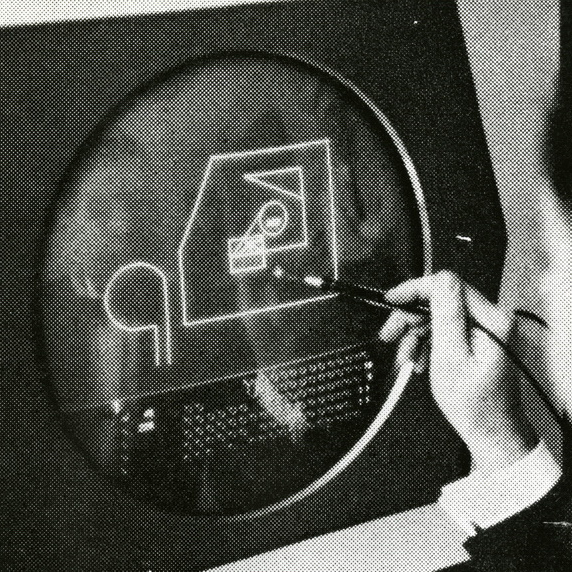
\includegraphics[width=8cm]{figuras/figura-1}}
		}{
			\Fonte{http://i0.wp.com/www.designleap.org/wp-content/uploads/2014/06/Sketchpad-Ivan-Sutherland-1963.jpg?resize=572\%2C572}
		}	
	\end{figure}
	\nocite{figura1}
	
Com o avanço resultado da criação dos circuitos integrados, cujo uso nos microprocessadores proporcionou um espantoso crescimento da indústria, os computadores deixaram de ser um monopólio das grandes companhias e tornaram-se muito mais acessíveis a pessoas simples. Isso abriu várias possibilidades para o mercado de computadores pessoais, entre elas destaca-se o surgimento das primeiras placas gráficas produzidas pela IBM (\acrlong{IBM}).

    \begin{figure}[h!]
		\centering
		\Caption{\label{fig:exemplo-2} Placa gráfica denominada Color Graphics Adapter produzida nos anos 80 pela IBM.}	
		\UNIFORfig{}{
			\fbox{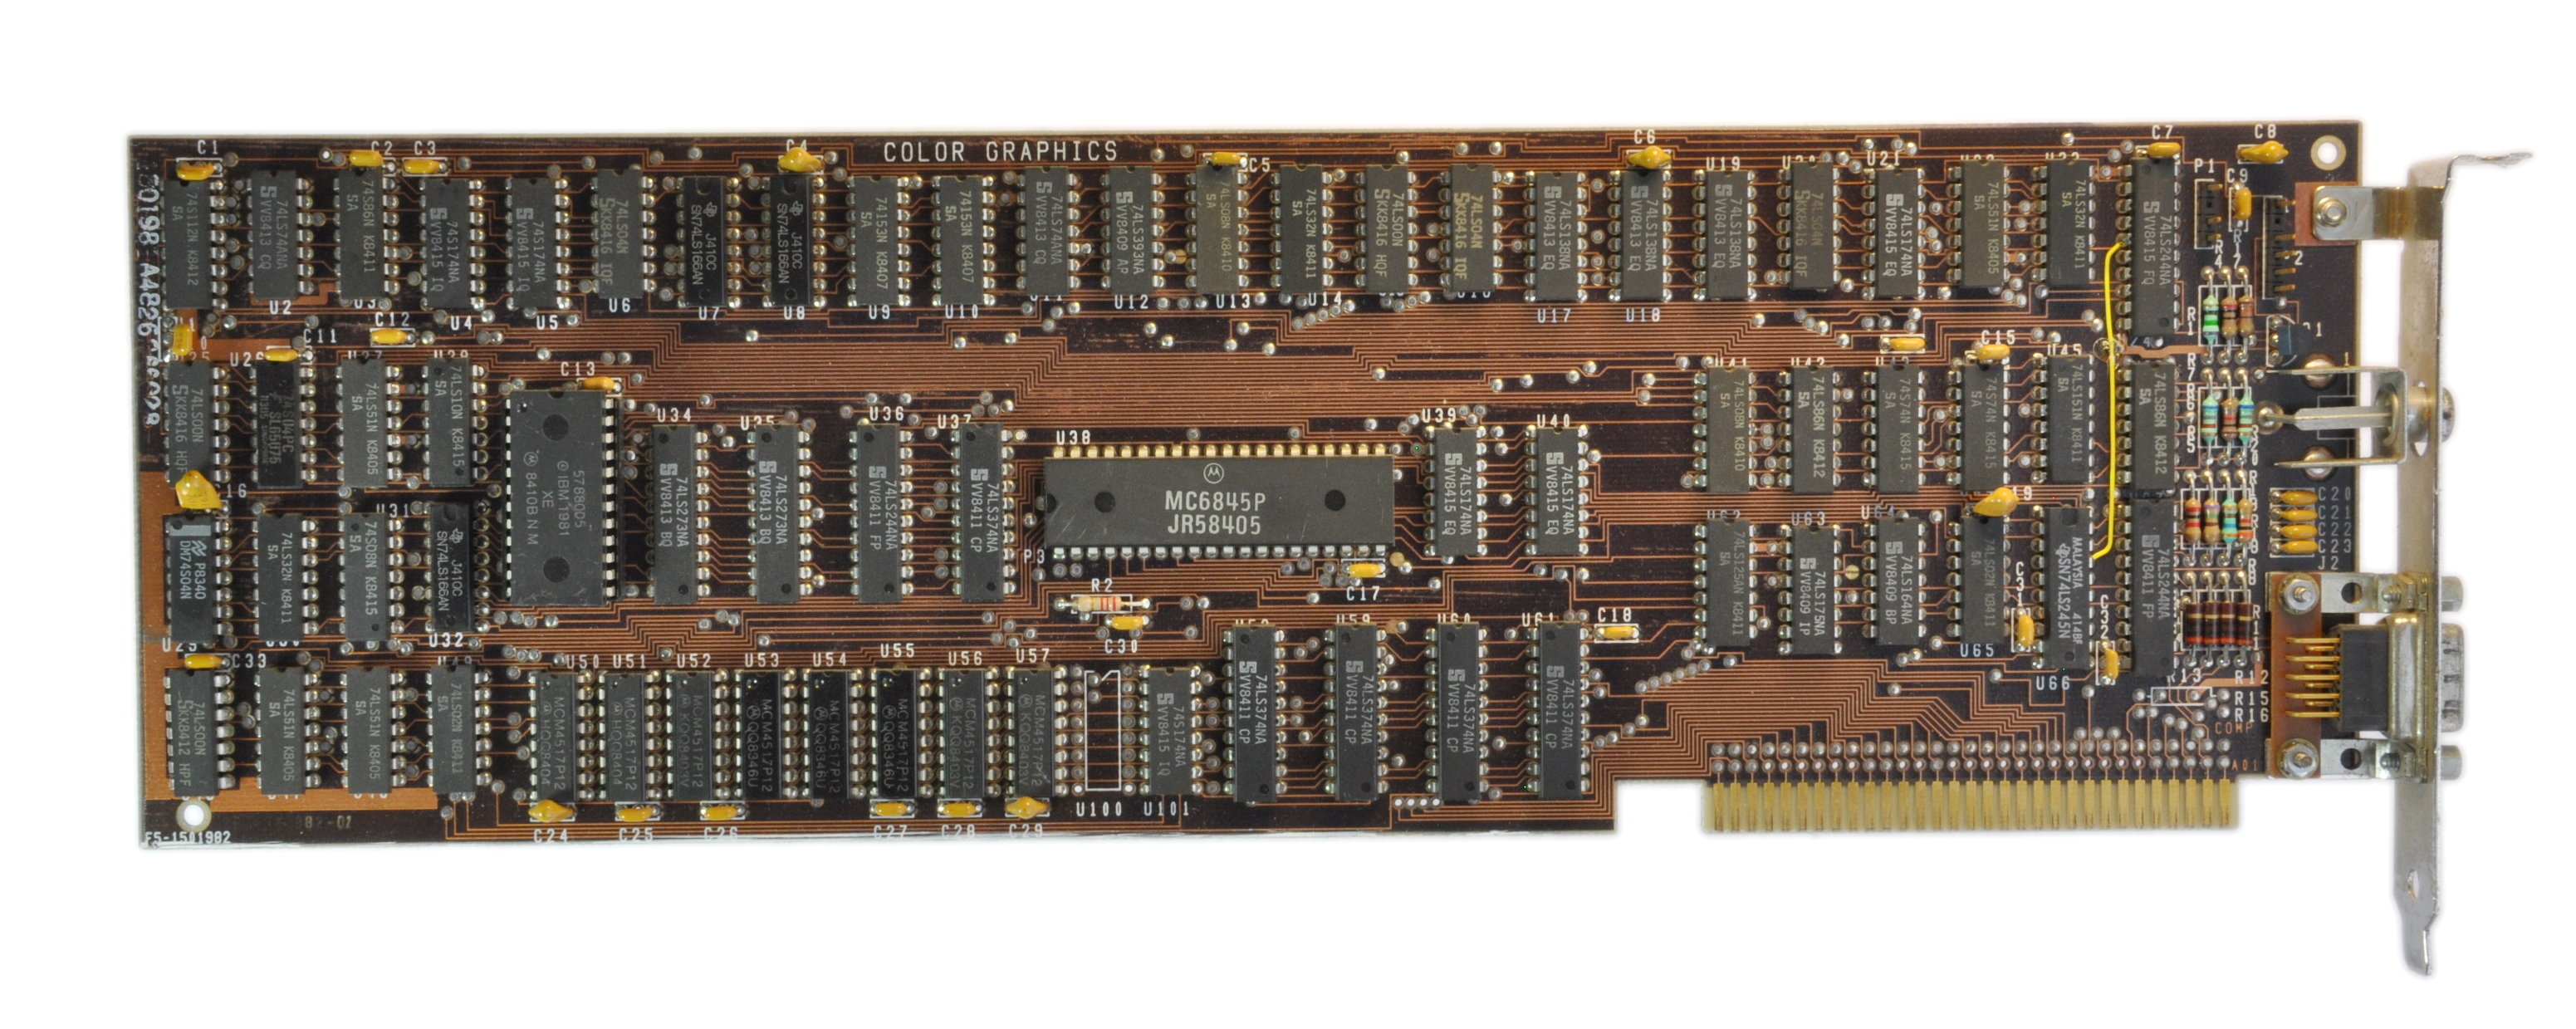
\includegraphics[width=15cm]{figuras/figura-2}}
		}{
			\Fonte{https://upload.wikimedia.org/wikipedia/commons/5/55/IBM\_Color\_Graphics\_Adapter.jpg}
		}	
	\end{figure}
	\nocite{figura2}
	
Como a indústria de jogos eletrônicos tinha mais recursos para explorar devido às melhorias de hardware disponíveis, vários jogos começaram a se destacar no mercado. Entre eles os mais marcantes para a popularização do uso de tecnologia de computação gráfica tridimensional foram lançados pela empresa id Software na década de 90. O primeiro sendo Wolfenstein 3D (que na realidade utilizava o modo 7 do Super NES (\acrlong{NES}) para emular a ambientação tridimensional) que definiu o padrão para jogos no gênero de tiro em primeira pessoa em 3D e o segundo sendo Doom que fazia uso de renderização com perspectiva 3D em tempo real por meio de software proprietário desenvolvido pela própria id Software voltado para produção com destino a computadores que utilizavam o sistema operacional da Microsoft (\acrshort{MS-DOS}).

    \begin{figure}[h!]
		\centering
		\Caption{\label{fig:exemplo-3} No lado esquerdo percebe-se que Doom fazia uso de 3D real enquanto no lado direito Wolfenstein posicionava imagens 2D em diferentes camadas para simular a profundidade tridimensional.}	
		\UNIFORfig{}{
			\fbox{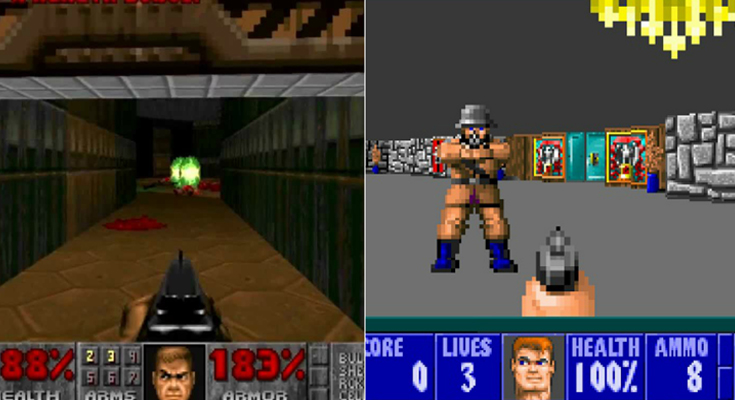
\includegraphics[width=13cm]{figuras/figura-3}}
		}{
			\Fonte{https://www.retrorefurbs.com/wolfenstein-vs-doom-the-battle-of-the-first-person-shooters/}
		}
	\end{figure}
	\nocite{figura3}
	
Paralelo ao cenário desses jogos \cite{openGLBook}, a Silicon Graphics (\acrshort{SGI}), uma companhia especializada em computação gráfica 3D e líder de mercado na época, trabalhava no lançamento open source da Open Graphics Library (\acrshort{OpenGL}), uma API (\acrlong{API}) padronizada multiplataforma de processamento de gráficos de computador em tempo real que rapidamente dominou o mercado, e que era uma derivação de outra biblioteca proprietária da mesma empresa, a IRIS GL (\acrlong{IRIS GL}). 

Vendo uma oportunidade de mercado, a Microsoft logo agiu e comprou a empresa RenderMorphics, criadora da \acrshort{API} Reality Lab, que teve o nome alterado para Direct3D e foi distribuido como um SDK (\acrlong{SDK}) conhecido como DirectX \cite{openGLBook}, acabando por se tornar o concorrente direto da \acrshort{OpenGL}. Essa rivalidade no final das contas acabou sendo benéfica tanto para o mercado de jogos eletrônicos quanto para os seus consumidores, já que acelerou o desenvolvimento de novas tecnologias que exploravam ao máximo o potencial do hardware disponível.
	
Mais adiante, em 1999, a empresa NVIDIA foi responsável for trazer mais uma inovação ao mercado, a "primeira GPU" (\acrlong{GPU}) foi como ficou conhecida a placa gráfica GeForce 256 (Figura 4), que fazia uso de uma tecnologia chamada T\&L (\acrlong{T+L}) que basicamente movia os cálculos de transformação e iluminação de vértices da CPU (\acrlong{CPU}) para a \acrshort{GPU}. Isso permitia uma maior velocidade em operações matemáticas de ponto flutuante. Então nos próximos anos o que se viu foi um crescimento exponencial de performance de \acrshort{GPU} para renderização em tempo real.

    \begin{figure}[h!]
		\centering
        \Caption{\label{fig:1} Hardware da placa gráfica da NVIDIA.}
        \begin{subfigure}{0.50\textwidth}
        \UNIFORfig{}{
			\fbox{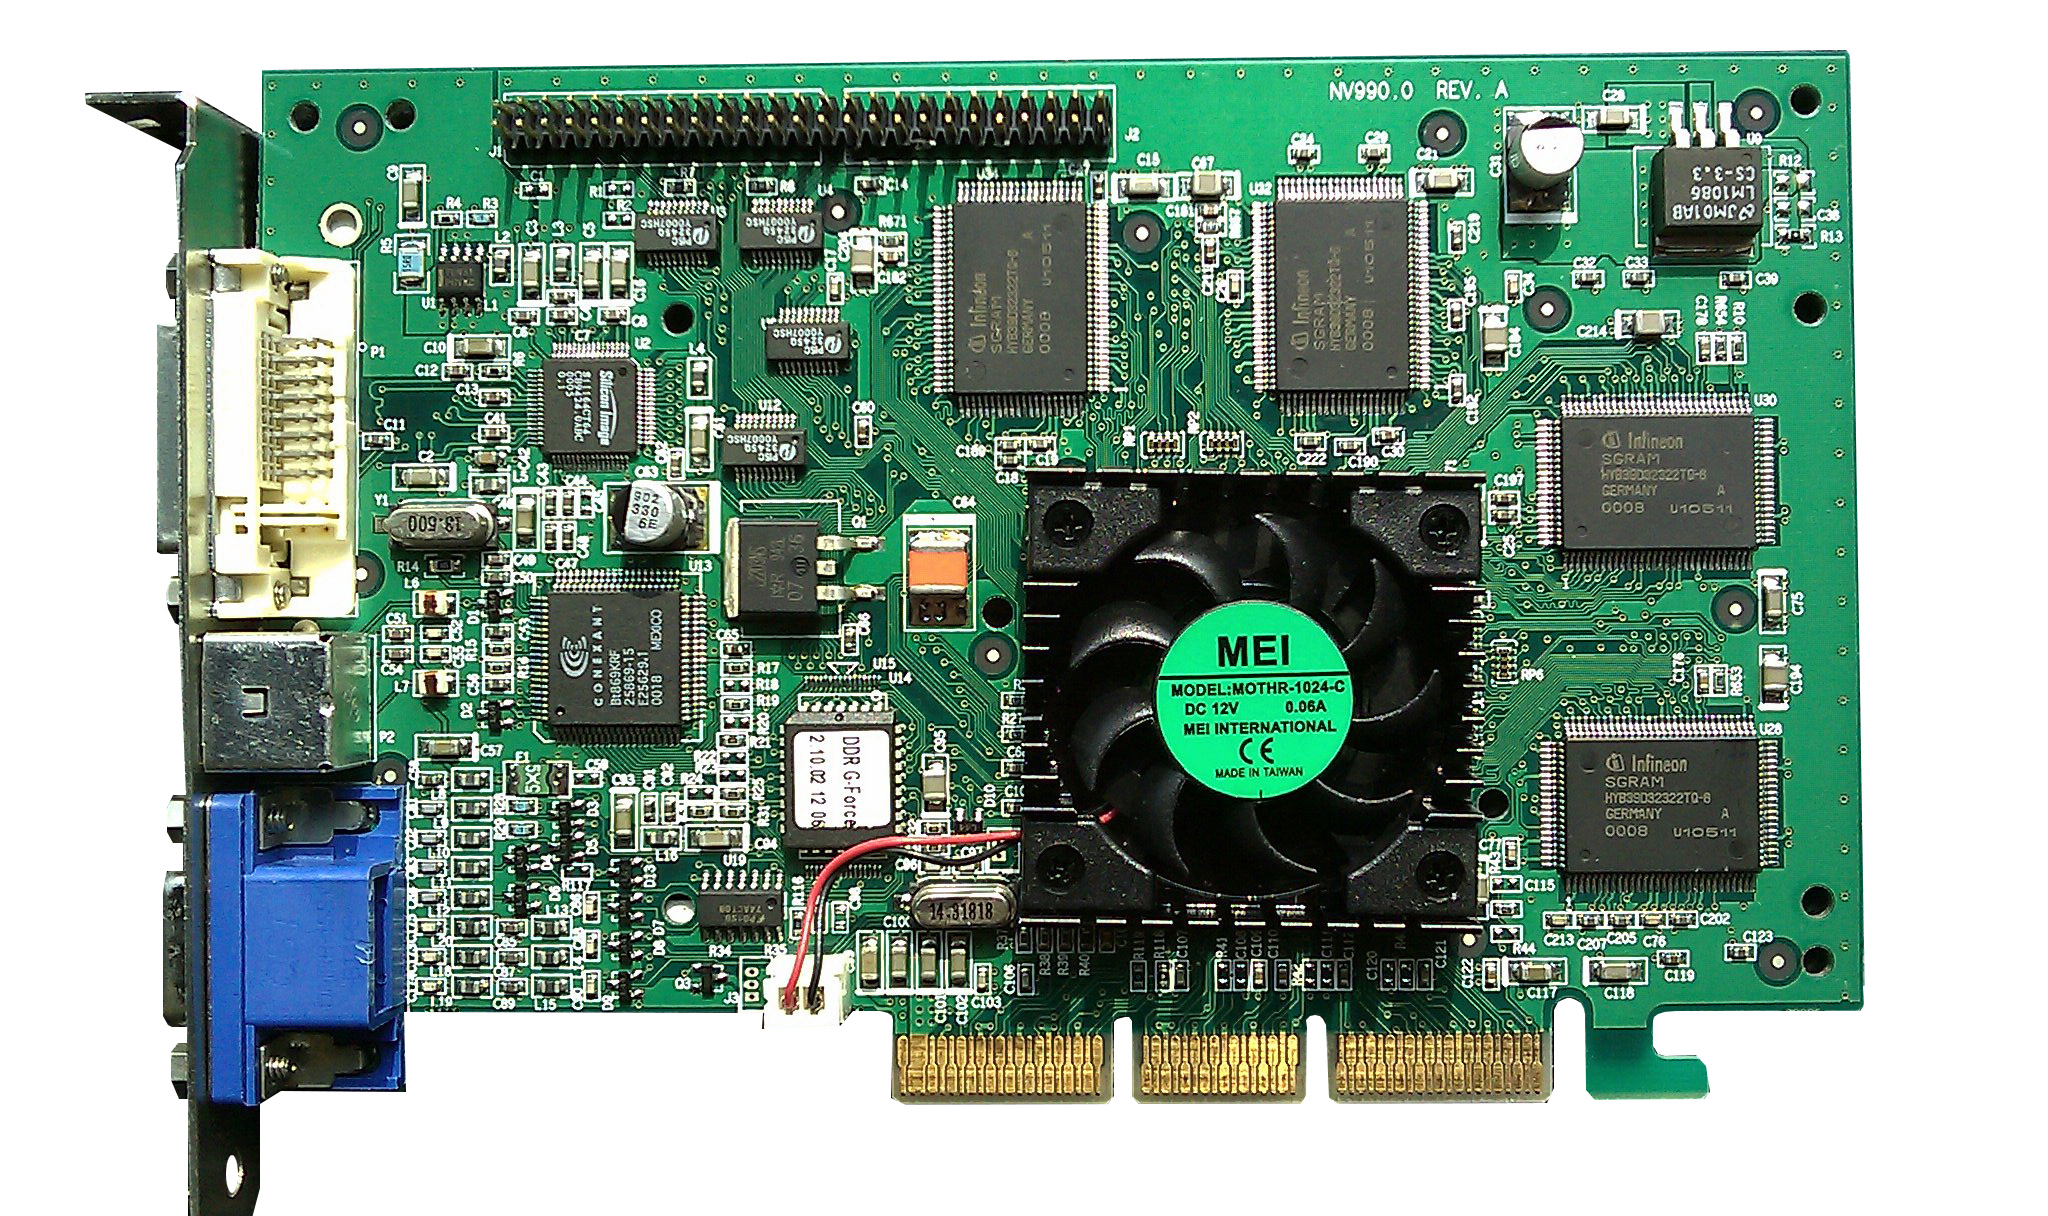
\includegraphics[width=\linewidth]{figuras/fig-a}}
		}{
		    \caption{GeForce 256} \label{fig:1a}
		}
		\nocite{figura4a}
        \end{subfigure}%
        
        \begin{subfigure}{0.30\textwidth}
        \UNIFORfig{}{
			\fbox{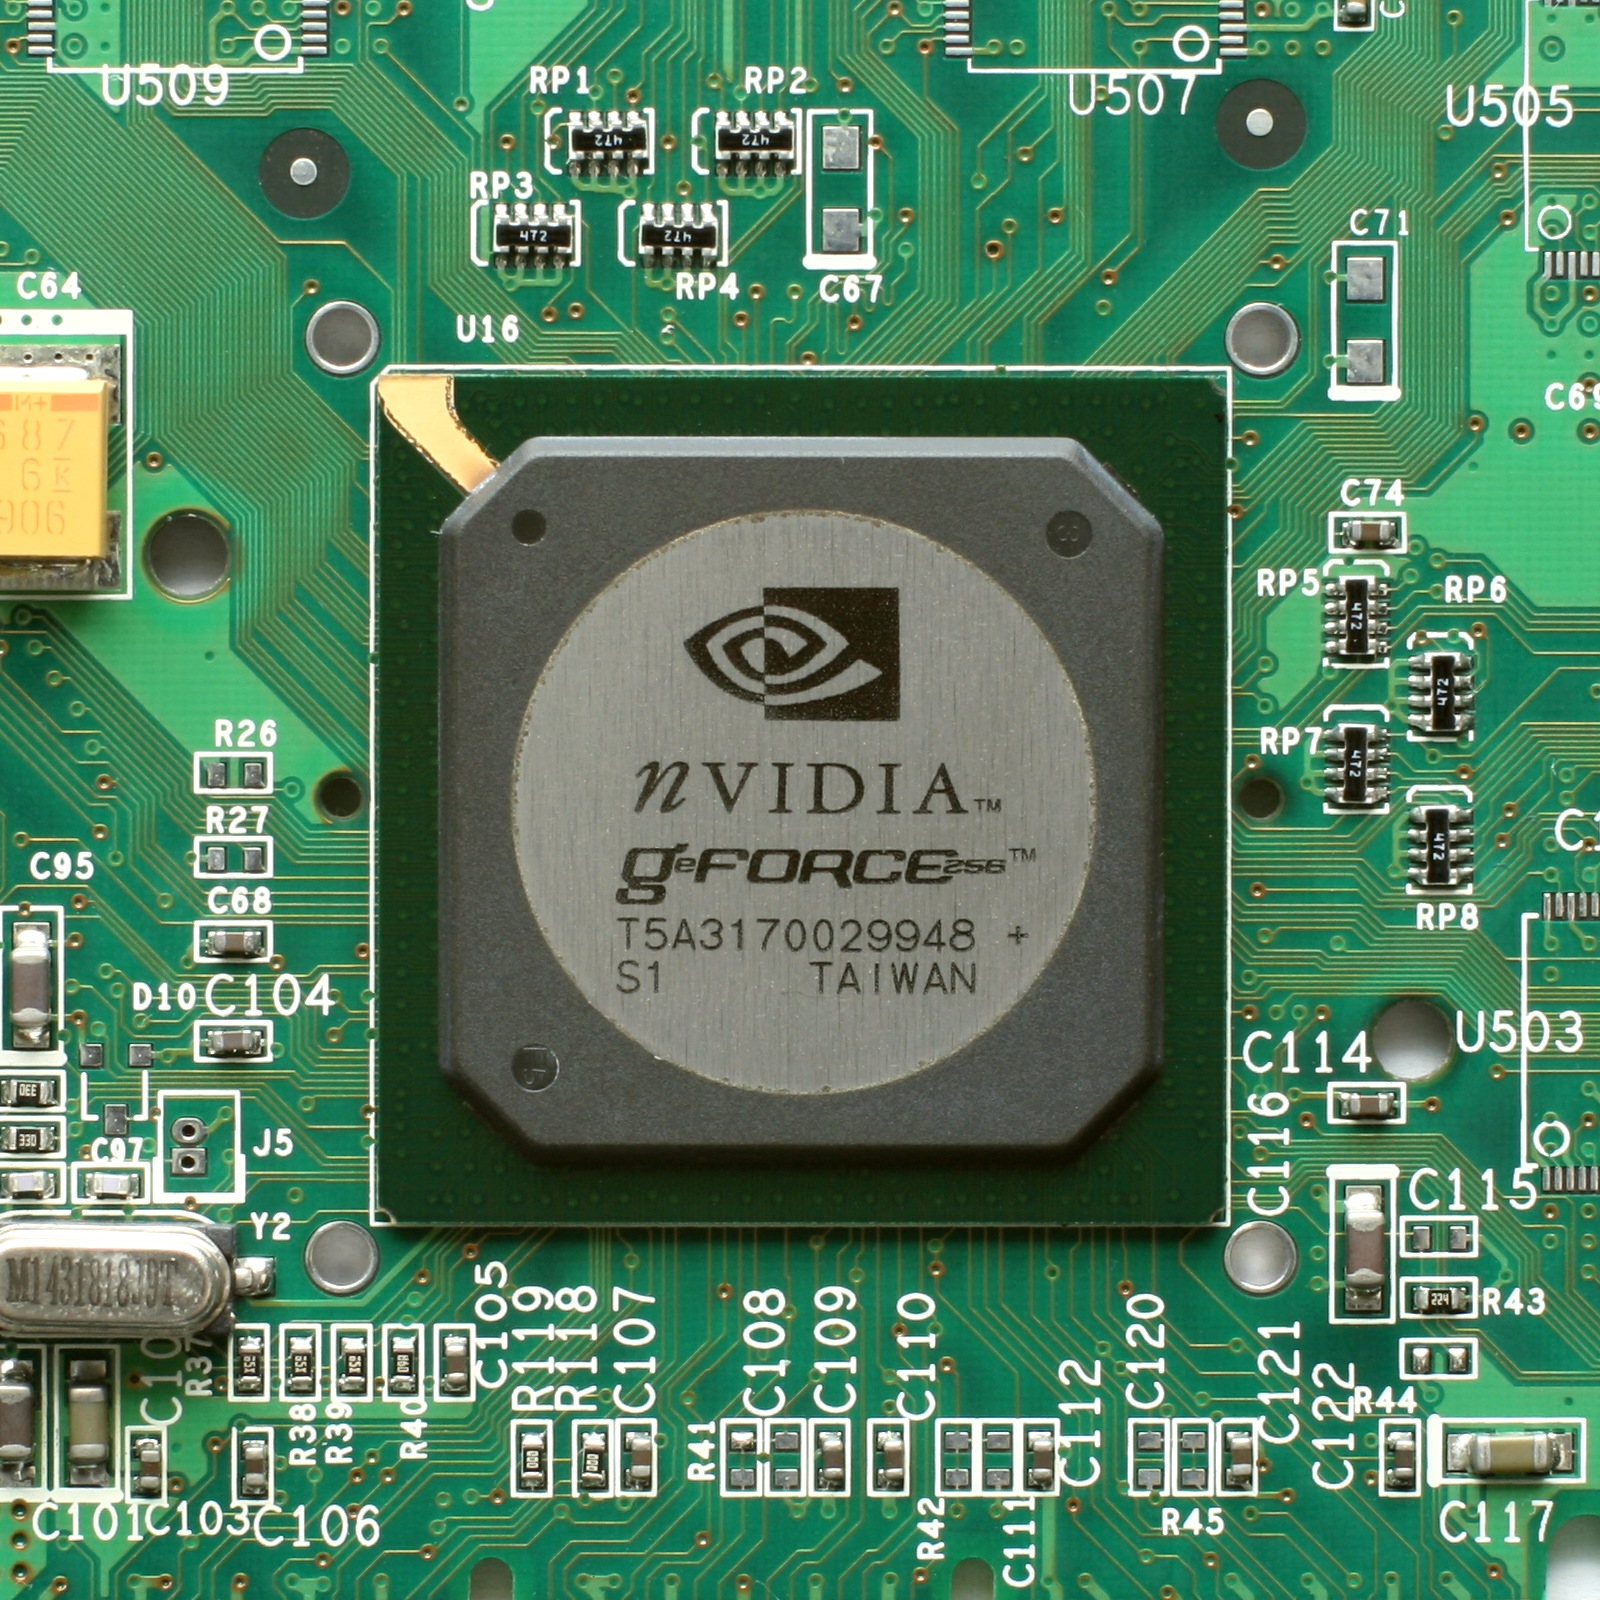
\includegraphics[width=\linewidth]{figuras/fig-b}}
		}{
		    \caption{GPU da GeForce 256} \label{fig:1b}
		}
		\nocite{figura4b}
        \end{subfigure}
		{
			\Fonte{https://upload.wikimedia.org/wikipedia/commons}
		}
	\end{figure}
	
Até então shaders eram bem vistos e utilizados por melhorar a performance eliminando carga de trabalho excessiva da \acrshort{CPU}, porém sua programação era difícil uma vez que a sintaxe utilizada era semelhante à programação em Assembly. Percebendo esse problema, a Microsoft, em 2003, lançou a versão 9.0 do Direct3D que trazia consigo a implementação da HLSL (\acrlong{HLSL}) que como o nome sugere permitia a programação de shaders em alto nível e possuia uma sintaxe bastante parecida com C. Enquanto isso, OpenGL também trouxe a sua própria linguagem de alto nível chamada GLSL (\acrlong{GLSL}) para competir no mercado \cite{openGLBook}. 

\subsection{Como o OpenGL funciona}
\label{sec:como-opengl-funciona}

Grosso modo, a API do OpenGL desenha gráficos em uma memória especializada em quadros de imagem (frame buffer) e os lê novamente quando precisa. O seu design único oferece suporte tanto a geometrias 3D quanto a imagens simples. O modelo de funcionamento dessa API pode ser descrito como cliente-servidor, pois a aplicação (cliente) faz solicitações por meio de comandos que são interpretados e processados pela implementação OpenGL (servidor) \cite{GLSLBook}. Aqui cabe destacar que a sincronia entre cliente e servidor e suas informações/dados não ocorre quando um comando é executado mas sim quando ele é emitido.

Os comandos são sempre processados na ordem em que são recebidos pelo servidor (execução fora de ordem não é permitida). Os dados passados para um comando OpenGL são então interpretados e copiados em memória caso seja necessário e as modificações subsequentes feitas pela aplicação não surtem efeito nos dados que estão armazenados internamente pelo OpenGL. Esses procedimentos são uma forma de garantir que um primitivo --- segundo Abdala (2019)\nocite{abdala}, uma representação discreta em grade de um elemento geométrico fundamental, e.g. ponto, linha, círculo, etc. --- seja desenhado apenas se o primitivo anterior houver sido completamente desenhado \cite{GLSLBook}.

OpenGL foi projetada para atuar como uma máquina de estados composta de parametros que definem o comportamento da pipeline de renderização e da forma que as primitivas são transformadas em pixels na tela. O estado é composto por uma estrutura de dados chamada contexto gráfico que é gerenciada pelo sistema de janelas do SO (\acrlong{SO}). O principio básico de funcionamento dessa API é transformar dados vindos de uma aplicação em algo visível na tela, esse processo é chamado de renderização e normalmente é acelerado por um hardware com design específico chamado de acelerador gráfico, entretanto suas operações podem ser parcial ou totalmente implementadas por software executado pela CPU. Aceleradores gráficos tipicamente possuem região de memória delimitada para manutenção do conteúdo exibido na tela, sendo que cada pixel é representado por uma quantidade de bytes na memória; uma tela em escala de cinza, por exemplo, pode fazer uso de um byte para representar a tonalidade de cinza de cada pixel \cite{GLSLBook}.

Essa região conhecida como memória de exibição é escaneada "x" vezes por segundo para eliminar a cintilação. Há ainda uma região específica para manipular dados que não são visíveis na tela chamada de memoria de não exibição. O responsável pela alocação de memória é o próprio sistema operacional que suporta o OpenGL. Em um sistema de janelas, a janela que corresponde a região da memória gráfica que é modificada durante a renderização é chamada de frame buffer. Já em um cenário sem janelas (i.e. tela cheia) o frame buffer corresponde a toda a tela \cite{GLSLBook}.

Para que uma janela consiga suportar a renderização ela precisa de uma combinação de alguns elementos: até quatro buffers para as cores, um buffer de profundidade (Figura 5), um \textit{stencil buffer} (Figura 6), um buffer de acumulação, um \textit{multisample buffer} e um ou mais buffers auxiliares. A maioria dos hardwares suporta o carregamento duplo, técnica que faz uso de um buffer frontal e um buffer posterior para que o processo de renderização seja realizado em plano de fundo e então quando terminar seu conteúdo é trocado com o do buffer frontal para exibir o resultado final e iniciar a nova renderização. Isso ajuda a conseguir animações suaves à taxas interativas \cite{GLSLBook}.

    \begin{figure}[h!]
		\centering
		\Caption{\label{fig:exemplo-6} O buffer de profundidade é mostrado em tons de cinza sendo que objetos próximos ficam com tonalidade mais escura enquanto objetos distantes assumem uma tonalidade mais clara.}	
		\UNIFORfig{}{
			\fbox{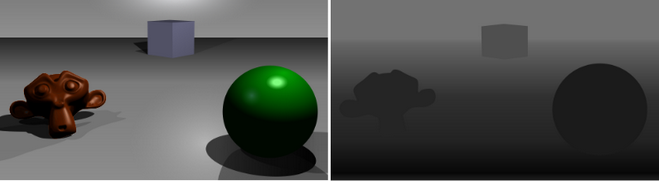
\includegraphics[width=15cm]{figuras/figura-6}}
		}{
			\Fonte{https://larranaga.github.io/Blog/imagenes/z-buffer.png}
		}
	\end{figure}
	\nocite{dptbuf}
	
No caso do suporte a visualização 3D estéreo, mais dois buffers serão utilizados em conjunto com os dois citados anteriormente para criar uma combinação com quatro buffers de cor que são divididos para cada olho. Se um objeto 3D precisa ser desenhado com remoção de superfície encoberta, o buffer de profundidade entra em ação comparando o valor da profundidade de cada pixel dos objetos em cena para determinar qual será visível ou obscurecido. E há ainda a opção do uso de um \textit{stencil buffer} para aplicar operações complexas utilizando máscaras com o objetivo de determinar onde cada pixel deve ser atualizado ou não \cite{GLSLBook}.

    \begin{figure}[h!]
		\centering
		\Caption{\label{fig:exemplo-7} O stencil buffer permite a customização da forma como objetos 3D são renderizados.}	
		\UNIFORfig{}{
			\fbox{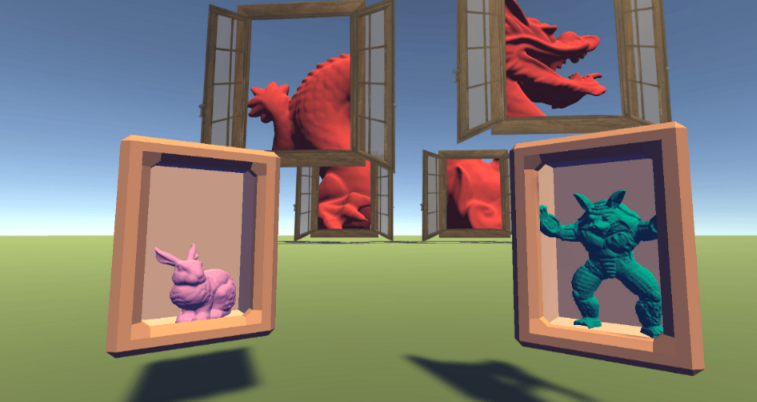
\includegraphics[width=15cm]{figuras/figura-7}}
		}{
			\Fonte{https://www.ronja-tutorials.com/assets/images/posts/022/Result.gif}
		}
	\end{figure}
	\nocite{stcbuf}

O buffer de acumulação é capaz de reproduzir efeitos complexos como suavização em tela cheia de alta qualidade, profundidade de campo e desfoque de movimento. Ele funciona como um buffer de cor, porém com maior precisão, capaz de acumular imagens para produzir uma úncia imagem composta. Seguindo essa linha, o \textit{multisample buffer} é capaz de produzir várias amostras da renderização para realizar suavização sem precisar renderizar a cena mais de uma vez \cite{GLSLBook}. Por último, os buffers auxiliares (mais de um pode ser utilizado) servem para guardar dados genéricos.

\subsubsection{Pipeline gráfica do OpenGL}
\label{sec:pipeline-opengl}

Para que a máquina de estados do OpenGL possa operar corretamente, foi definida uma ordem específica em que as operações envolvidas no processo de renderização precisam ser realizadas, essa padronização é chamada de \textit{pipeline} gráfica \cite{GLSLBook} e pode ser vista na Figura 7. Todos os dados necessários para desenhar a geometria estão contidos em espaço em memória e podem ser lidos pelo OpenGL de três maneiras diferentes. 

A primeira seria enviar um vértice de cada vez utilizando alguns comandos intermitentes para manipular atributos dos vértices. A segunda seria utilizar matrizes de vértices, o que oferece melhor performance devido a forma de organização dos dados, pois são utilizados ponteiros e mais dados podem ser processados de uma vez. Esses dois casos citados acima fazem uso do modo imediato pois as primitivas são renderizadas assim que são especificadas \cite{GLSLBook}. 

O terceiro modo seria utilizar algum dos dois procedimentos citados acima implementando uma lista de exibição, que é uma estrutura de dados que guarda comandos para execução futura. Algumas vantagens desse método no que diz respeito a performance seria a possibilidade de otimizar os comandos contidos na lista, ou ainda guardar os comandos na memória do acelerador gráfico para uma melhor performance de desenho \cite{GLSLBook}. 

	\begin{figure}[h!]
		\centering
		\Caption{\label{fig:pipeline} Pipeline gráfico do OpenGL.}	
		\UNIFORfig{}{
			\fbox{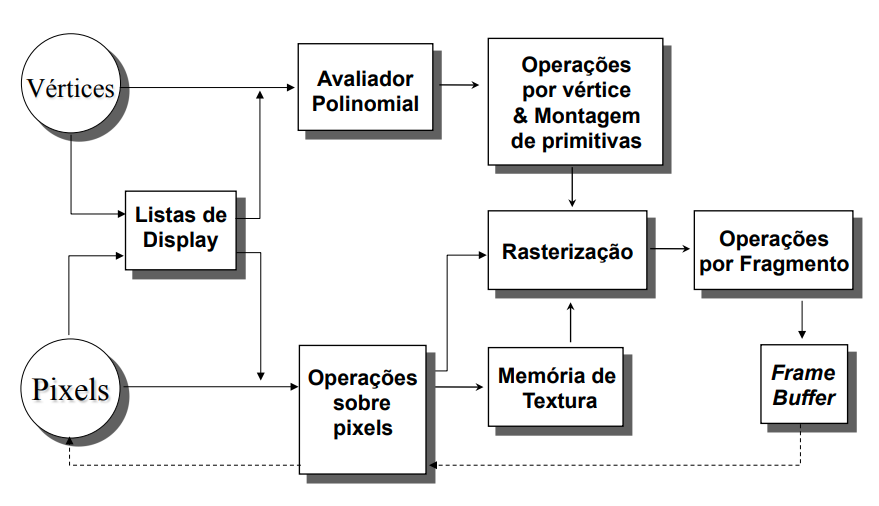
\includegraphics[width=15cm]{figuras/pipeline.png}}
		}{
			\Fonte{\url{http://www.ic.uff.br/~anselmo/cursos/CGI/slidesGrad/CG_aula4(introducaoaOpenGL).pdf}}
		}
	\end{figure}
	\nocite{pipeline}
	
Como todas as primitivas geométricas podem ser descritas por vértices, as curvas e as superfícies podem ser descritas pelas funções polinomiais chamadas funções base. A função do avaliador polinomial nesse caso é derivar os vértices para conseguir representar superfícies e curvas. Isso é feito através do método de mapeamento polinomial, que produz as normais da superfície, as coordenadas da textura, as cores, e valores de coordenadas espaciais dos pontos de controle (VIEIRA, 2017)\nocite{pipelnRef}.

A próxima etapa é o estágio das operações por vértice que converte os vértices em primitivas. Alguns dados do vértice são transformados em matrizes de pontos flutuantes. Nesta etapa ocorre a projeção de coordenadas do espaço do mundo para o espaço da tela. Inclui algumas etapas como geração e transformação de coordenadas de textura, e também cálculos de luz para produção dos valores de cor (VIEIRA, 2017). Por isso é normal que essa etapa exija mais recursos computacionais. 

Logo em seguida ocorre a montagem das primitivas por meio do \textit{clipping} (eliminação de parte da geometria desnecessária para a renderização), que é um processo onde se a primitiva está totalmente dentro do plano de visualização ela é repassada para o devido processamento. Caso ela esteja totalmente fora do plano de visualização ela é rejeitada e não é processada. Se a primitiva estiver parcialmente visível no plano, ela é dividida para que somente a porção visível siga para processamento.

Outra operação que ocorre nesse estágio é a projeção das coordenadas da perspectiva para coordenadas da janela. Além disso, há ainda uma etapa opcional de \textit{culling} onde os polígonos são testados para saber se será preciso descartar faces posteriores, anteriores ou ambas \cite{GLSLBook}. Paralelamente a esse processo, os dados de pixels contidos em uma matriz na memória do sistema são empacotados e escalados, inclinados e processados por um mapa de pixels. Os resultados, que serão então empacotados em um formato apropriado e retornados a uma matriz de memória do sistema, podem ser escritos na memória da textura ou emitidos à uma etapa de rasterização.

Rasterização é a etapa de conversão de dados tanto geométricos como de pixel em fragmentos. Cada quadrado do fragmento corresponde a um pixel no \textit{frame buffer}, sendo que os valores da cor e da profundidade são atribuídos para cada um. Ao final são executadas mais algumas operações antes de armazenar os valores no \textit{frame buffer} como: \textit{texturing}, onde um elemento da textura é gerado e aplicado da memória da textura para cada fragmento; cálculos de névoa; testes de profundidade, transparência e remoção de faces ocultas (VIEIRA, 2017). Apesar dessa etapa possuir muitos processos, as operações são relativamente simples e podem ser executadas eficientemente para milhões de pixels por segundo com o hardware disponível atualmente.

Em relação a etapa de texturização, uma das mais complexas, é interessante destacar que a API tem capacidade de trabalhar com quatro tipos de texturas. Texturas de uma dimensão (vetor de pixels), texturas 2D (matriz $ mxn $ de pixels), texturas 3D (matriz com uma dimensão a mais para guardar informações adicionais e.g. profundidade), e mapas cúbicos (normalmente usado para simular reflexões de ambiente). A API também fornece métodos para trabalhar com formatos de imagem compactados, esses usam significativamente menos memória e melhoram a performance \cite{GLSLBook}.

É importante destacar que a API também fornece a possibilidade de utilizar texturas do tipo \textit{mipmap} --- várias representações da mesma imagem, porém cada uma tem metade da resolução da anterior --- em conjunto com o parâmetro de nível de detalhe que será detalhado mais adiante, mas que de forma simplificada permite a otimização do processo de renderização de objetos que estão distantes da câmera. 

\subsubsection{Matrizes de transformação de coordenadas}
\label{sec:matrizes-transformacao-coordenadas}

Esse é um tópico mais complexo, mas que também é importante para entender como a pipeline gráfica do OpenGL transforma descrições de objetos tridimensionais em imagens 2D que são exibidas na tela (Figura \ref{fig:spaces}). Algo semelhante a como uma câmera pode ser usada para criar uma representação em imagem de algo no mundo real. Entretanto nesse caso o primeiro passo consiste em pegar as informações do modelo do objeto 3D, como posição dos vértices e normais da superfície, para interpretá-las como coordenadas do espaço do objeto \cite{GLSLBook}. 

	\begin{figure}[htp]
		\centering
		\Caption{\label{fig:spaces} Processo de transformação entre os sistemas de coordenadas e seus espaços.}	
		\UNIFORfig{}{
			\fbox{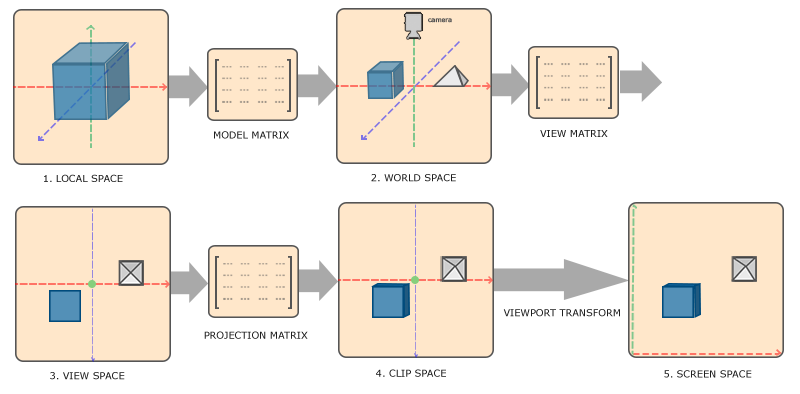
\includegraphics[width=12cm]{figuras/spaces.png}}
		}{
			\Fonte{\url{https://learnopengl.com/img/getting-started/coordinate_systems.png}}
		}
	\end{figure}
	\nocite{spaces}

Como cada objeto tem suas próprias características é necessário definir um sistema de coordenadas uniforme para que seja possível usar vários objetos em uma única cena. Para isso é utilizado o sistema de coordenadas global, e aqui a API vai um passo além e realiza mais uma conversão para o sistema de coordenadas de olho levando em consideração a posição da câmera na cena, seu ponto focal (para onde a câmera está olhando) e o vetor de direção para cima (e.g. a orientação da câmera) \cite{GLSLBook}. 

	\begin{equation}
		\begin{bmatrix}
			x_{olho} \\
			y_{olho} \\
			z_{olho} \\
			w_{olho} \\
		\end{bmatrix}
		=
		M_{modelView} \cdot
		\begin{bmatrix}
			x_{obj} \\
			y_{obj} \\
			z_{obj} \\
			w_{obj} \\
		\end{bmatrix}
	\end{equation}

Na equação 2.1, a matriz \textit{modelView} é uma multiplicação das matrizes de conversão de coordenadas de espaço de objeto para espaço global e de espaço global para espaço de olho. O cálculo das normais é semelhante, a diferença é que é utilizada a matriz transposta da inversa da matriz \textit{modelView} para multiplicar um vetor de normais. Como é possível ver na Figura \ref{fig:worldview} os três elementos mais à direita ($ m_{12} $, $ m_{13} $, $ m_{14} $) são para transformação de translação. O $ m_{15} $ é uma coordenada homogênea (Apêndice --- A) usada para transformação para o espaço de projeção. Os três conjunto de elementos ($ m_{0} $, $ m_{1} $, $ m_{2} $), ($ m_{4} $, $ m_{5} $, $ m_{6} $) e ($ m_{8} $, $ m_{9} $, $ m_{10} $) são usados para rotação e escala e representam os três eixos ortogonais x, y e z \cite{openglOnline}.

	\begin{figure}[h!]
		\centering
		\Caption{\label{fig:worldview} Conteúdo das quatro colunas da matriz \textit{modelView}.}	
		\UNIFORfig{}{
			\fbox{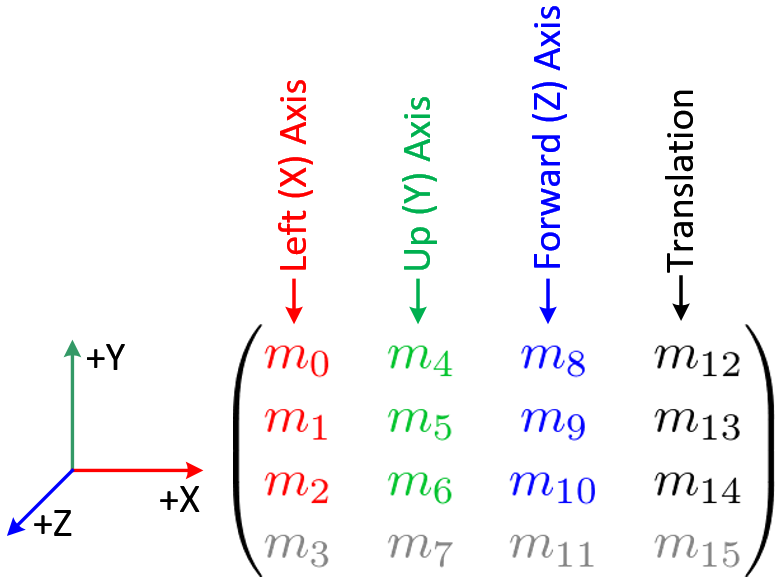
\includegraphics[width=7cm]{figuras/modelView.png}}
		}{
			\Fonte{\url{http://www.songho.ca/opengl/gl_transform.html}}
		}
	\end{figure}

Após essa conversão, as coordenadas obtidas são multiplicadas pela matriz de projeção para definir como os vértices serão projetados na tela, os valores dessa matriz dependem se modo de projeção utilizado é em perspectiva ou ortográfico (Figura \ref{fig:frustum}) e são mostrados nas equações \ref{eq-persp} e \ref{eq-ortho} respectivamente. 

	\begin{equation} \label{eq-persp}
		\resizebox{.35\hsize}{!}{$ M_{persp}
		=
		\begin{bmatrix}
			\cfrac{2n}{r-l} & 0 & \cfrac{r+l}{r-l} & 0 \\
			0 & \cfrac{2n}{t-b} & \cfrac{t+b}{t-b} & 0 \\
			0 & 0 & \cfrac{-(f+n)}{f-n} & \cfrac{-2fn}{f-n}\\
			0 & 0 & -1 & 0 \\
		\end{bmatrix} $}
	\end{equation}
	\begin{equation} \label{eq-ortho}
		\resizebox{.35\hsize}{!}{$ M_{orto}
		=
		\begin{bmatrix}
			\cfrac{2}{r-l} & 0 & 0 & -\cfrac{r+l}{r-l} \\
			0 & \cfrac{2}{t-b} & 0 & -\cfrac{t+b}{t-b} \\
			0 & 0 & \cfrac{-2}{f-n} & -\cfrac{f+n}{f-n}\\
			0 & 0 & 0 & 1 \\
		\end{bmatrix} $}
	\end{equation}

Os valores obtidos nessa operação são normalizados em uma região cúbica definida pelos pontos (-1, -1, -1) e (1, 1, 1) para espaço de coordenadas de dispositivo normalizado, isso significa que os valores passam a ser algum valor entre -1 e 1. Essa etapa é necessária para qua a área de visualização seja apropriadamente mapeada em uma janela de exibição de tamanho arbitrário. Por último, as coordenadas são convertidas para o sistema de coordenadas de tela. A partir desse ponto elas continuam para o processo de rasterização da pipeline do OpenGL \cite{openglOnline}. 
	\begin{figure}[hbp]
		\centering
        \Caption{\label{fig:frustum} Modos de projeção de câmera. As letras correspondem a \textit{left, right, bottom, top, near e far}.}
        \begin{subfigure}{0.46\textwidth}
        \UNIFORfig{}{
			\fbox{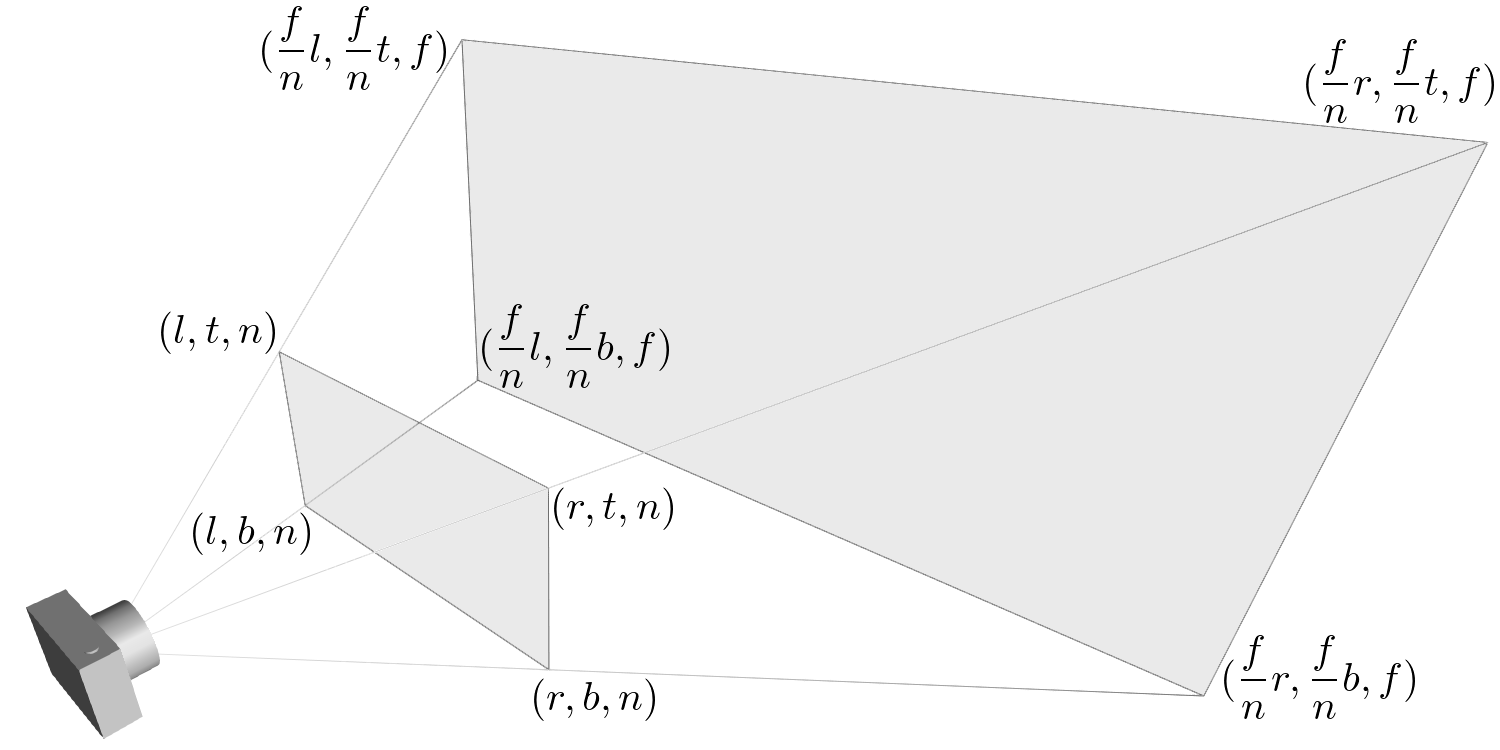
\includegraphics[width=\linewidth]{figuras/persp.png}}
		}{
		    \caption{\Gls{view-frustum} em perspectiva}
		}
        \end{subfigure}
		\hfill
        \begin{subfigure}{0.48\textwidth}
        \UNIFORfig{}{
			\fbox{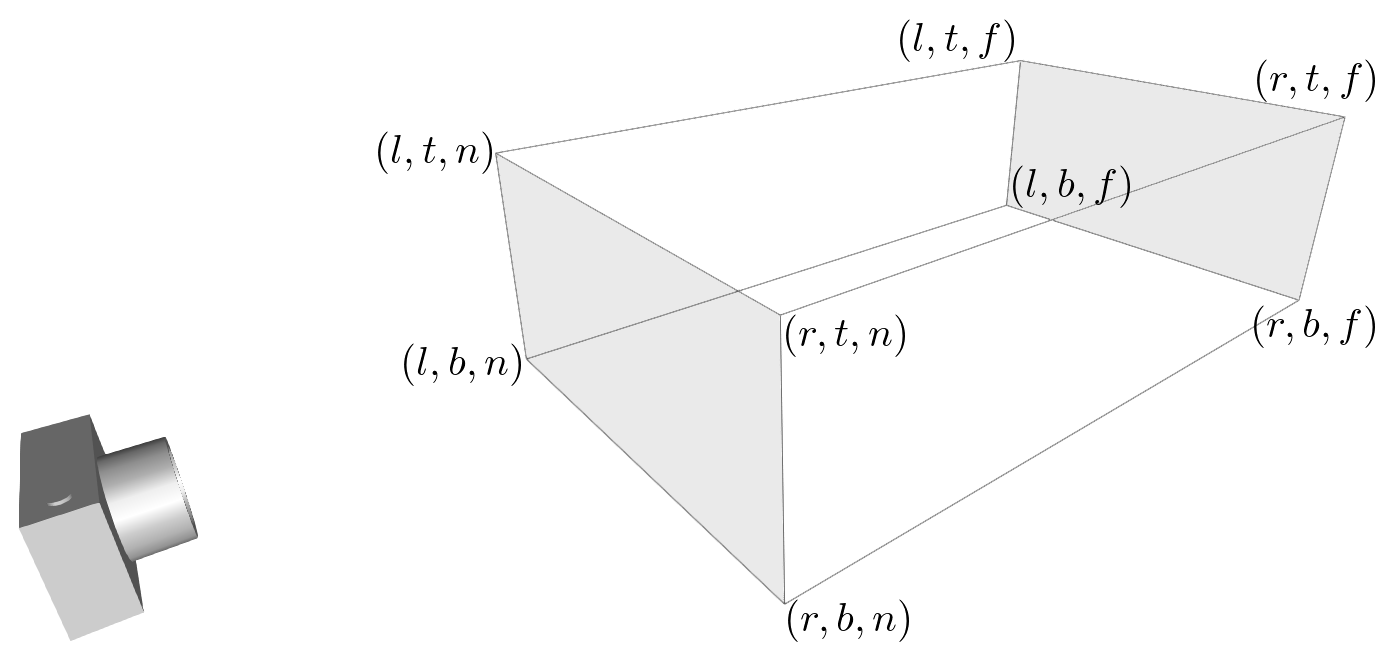
\includegraphics[width=\linewidth]{figuras/ortho.png}}
		}{
		    \caption{\Gls{view-frustum} ortográfico}
		}
        \end{subfigure}
		{
			\Fonte{\url{http://www.songho.ca/opengl/gl_transform.html}}
		}
	\end{figure}

\subsection{GLSL}
\label{sec:glsl}

Devido à necessidade crescente de substituir funcionalidades fixas por programabilidade em áreas que ficavam cada vez mais complexas, como processamento de vértices e fragmentos, foi desenvolvida uma solução que adicionou estágios programáveis para resolver esse problema. Essa solução foi a introdução da linguagem de sombreamento \acrshort{GLSL}, feita para ser executada nos dois processadores programáveis existentes no OpenGL: processador de vértices e processador de fragmentos (portanto os respectivos nomes \textit{vertex shader} e \textit{fragment shader}). Um shader pode então ser definido como um código escrito em uma linguagem de sombreamento (HLSL, GLSL, RSL e etc) com o propósito de ser executado por um dos processadores programáveis do OpenGL. Um programa de shader é então um conjunto de shaders compilados executáveis \cite{GLSLBook}.

GLSL faz uso de uma sintaxe bastante similar a linguagem de programação C. Seus tipos incluem vetores e matrizes por serem estruturas fundamentais para cálculos matemáticos com operações para gráficos 3D. Além disso, suporta laços, chamadas a sub-rotinas, expressões condicionais e conta com funções embutidas próprias para o desenvolvimento de shaders. Essa linguagem possibilitou aos desenvolvedores implementar um conjunto de diferentes técnicas para conseguir obter uma variedade enorme de efeitos visuais; não somente isso mas o fato de que essas técnicas são implementadas com aceleração via hardware pela GPU (com processamento paralelo) proporciona um aumento drástico de performance e libera carga da CPU para realizar outras tarefas \cite{GLSLBook}.

\subsection{HLSL}
\label{sec:hlsl}


\section{Aprofundando Conceitos Técnicos de Shaders}
\label{sec:aprofundando-conceitos-tecnicos-shaders}

Ao estudar computação gráfica a dúvida mais comum ao se deparar com certos termos utilizados é "o que é um shader". Essa palavra pode causar uma certa estranheza no início mas sua definição não é nenhum bicho de sete cabeças. Shaders são apenas pequenos programas (assim como um reprodutor de mídia ou uma calculadora de um computador) que são executados diretamente pela \acrshort{GPU} ao invés da \acrshort{CPU}. Isso permite a redução da carga de trabalho gráfico da \acrshort{CPU} pelo redirecionamento das tarefas para a \acrshort{GPU} que possui hardware especializado para isso \cite{openGLBook}.

	\begin{figure}[h!]
		\centering
		\Caption{\label{fig:exemplo-5} Demonstração de como é possível criar visuais únicos utilizando shaders.}	
		\UNIFORfig{}{
			\fbox{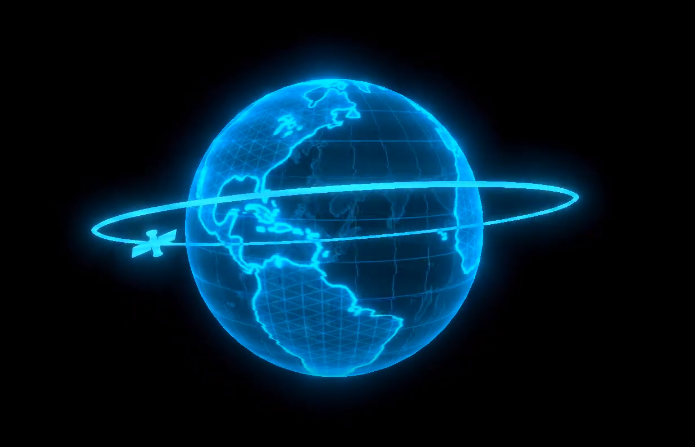
\includegraphics[width=12cm]{figuras/figura-5}}
		}{
			\Fonte{Adaptado de \url{https://www.youtube.com/watch?time_continue=2&v=F0CWzpYY68A&feature=emb_logo}}
		}
	\end{figure}
	\nocite{figura5}

Tecnicamente falando, um shader contém um conjunto de instruções que são executadas concorrentemente para cada pixel desenhado na tela. Essa forma de operação abre um leque de possibilidades, onde é possível por exemplo atribuir um comportamento para cada pixel baseado na sua posição na tela. Em uma comparação com programação procedural, ele funcionaria como uma função que recebe uma posição e retorna uma cor, sendo que após a compilação seu tempo de execução é extremamente rápido \cite{bookOfShaders}.

Uma metáfora para ajudar a compreender a dimensão da complexidade do processamento de um shader seria imaginá-lo como um bloco de várias tarefas que passa por uma linha de produção industrial. As tarefas podem ser pequenas ou grandes e consequentemente podem demandar mais processamento e energia. No caso da CPU cada trabalho seguinte teria que esperar o término do atual para começar \cite{bookOfShaders}. É interessante ressaltar que hoje em dia existe a tecnologia de multiprocessamento, onde os computadores normalmente possuem grupos de quatro processadores que atuam em conjunto para realizar as tarefas.

Considerando uma tela com resolução de 800x600, significa que 480.000 pixels precisam ser processados a cada frame sendo que normalmente é utilizada uma taxa de 30 frames por segundo (\acrshort{FPS}), então será necessário fazer 14.400.000 cálculos por segundo. Isso explica o fato de video games e outras aplicações gráficas exigirem muito mais poder de processamento que outros programas. Seu conteúdo gráfico implica em inúmeras operações por cada pixel, pois cada pixel na tela precisa ser computado, e também em perspectivas e geometrias de jogos 3D \cite{bookOfShaders}.  

Esse cenário pode ser suficiente para sobrecarregar um microprocessador comum e fica pior quando leva-se em consideração as tecnologias que fazem uso seja de taxa de FPS maior, seja de resoluções maiores como 2K, e acima. Para resolver esse problema utiliza-se processamento paralelo. A GPU possui vários pequenos microprocessadores que funcionam concorrentemente, além disso ela possui funções matemáticas específicas aceleradas via hardware para realizar operações matriciais e trigonométricas rapidamente \cite{bookOfShaders}.


\subsection{Vertex Shader}

A vertex shader is a GPU program that is executed once per vertex that is assigned to, and a pixel shader is a GPU program that is executed once per pixel.
Vertex processing involves the operations that occur at each vertex, most notably transformation and lighting. Fragments are per-pixel data structures that are created by the rasterization of graphics primitives. A fragment contains all the data necessary to update a single location in the frame buffer. Fragment processing consists of the operations that occur on a per-fragment basis, most notably reading from texture memory and applying the texture value(s) at each fragment \cite{GLSLBook}.

\subsection{Fragment Shader}





Nunc ac pretium dui. Mauris aliquam dapibus nulla ac mattis. Aenean non tortor volutpat, varius lectus vitae, accumsan nibh. Cras pretium vestibulum enim, id ullamcorper tortor ultrices non. Integer sodales viverra faucibus. Curabitur at dui lacinia, rhoncus lacus at, blandit metus. Integer scelerisque non enim quis ornare.

\lipsum[13]

	\begin{table}[h!]	
		\centering
		\Caption{\label{tab:exemplo-3} Duis faucibus, enim quis tincidunt pellentesque, nisl leo varius nulla, vitae tempus dui mauris ac ante purus lorem}		
		\UNIFORtab{}{
			\begin{tabular}{cll}
				\toprule
				Ranking & Exon Coverage & Splice Site Support \\
				\midrule \midrule
				E1 & Complete coverage by a single transcript & Both splice sites\\
				E2 & Complete coverage by more than a single transcript & Both splice sites\\
				E3 & Partial coverage & Both splice sites\\
				E4 & Partial coverage & One splice site\\
				E5 & Complete or partial coverage & No splice sites\\
				E6 & No coverage & No splice sites\\
				\bottomrule
			\end{tabular}
		}{
		\Fonte{Elaborado pelo autor}
	}
	\end{table}

Duis faucibus, enim quis tincidunt pellentesque, nisl leo varius nulla, vitae tempus dui mauris ac ante. Quisque purus lorem, pharetra sit amet lobortis eu, vehicula vitae purus. Ut varius, erat nec vehicula elementum, risus est tempus justo, nec vulputate augue leo egestas metus.

\lipsum[14]

	\begin{table}[h!]	
		\centering
		\Caption{\label{tab:exemplo-5} Etiam molestie, nulla a egestas aliquet, velit augue congue metus}		
		\UNIFORtab{}{
			\begin{tabular}{ccll}
				\toprule
				Quisque & pharetra & tempus & vulputate \\
				\midrule \midrule
				E1 & Complete coverage by a single transcript & Both splice sites\\
				E2 & Complete coverage by more than a single transcript & Both splice sites\\
				E3 & Partial coverage & Both splice sites & Both \\
				E4 & Partial coverage & One splice site & Both \\
				E5 & Complete or partial coverage & No splice sites & Both\\
				E6 & No coverage & No splice sites\\
				\bottomrule
			\end{tabular}
		}{
		\Fonte{Elaborado pelo autor}
	}
	\end{table}
	
	%como usar as siglas e abreviações
	%\acrlong{MIT}
	\acrlong{MIT}

\begin{alineascomponto}
	\item Integer non lacinia magna. Aenean tempor lorem tellus, non sodales nisl commodo ut
	\item Proin mattis placerat risus sit amet laoreet. Praesent sapien arcu, maximus ac fringilla efficitur, vulputate faucibus sem. Donec aliquet velit eros, sit amet elementum dolor pharetra eget
	\item Integer eget mattis libero. Praesent ex velit, pulvinar at massa vel, fermentum dictum mauris. Ut feugiat accumsan augue, et ultrices ipsum euismod vitae
	\begin{subalineascomponto}
		\item Integer non lacinia magna. Aenean tempor lorem tellus, non sodales nisl commodo ut
		\item Proin mattis placerat risus sit amet laoreet.
	\end{subalineascomponto}
\end{alineascomponto}
	\chapter{Trabalhos Relacionados}
\label{cap:trabalhos-relacionados}

Integer non lacinia magna. Aenean tempor lorem tellus, non sodales nisl commodo ut. Proin mattis placerat risus sit amet laoreet. Praesent sapien arcu, maximus ac fringilla efficitur, vulputate faucibus sem. Donec aliquet velit eros, sit amet elementum dolor pharetra eget. Integer eget mattis libero

\section{Trabalho Relacionado A}
\label{sec:trabalho-relacionado-a}

\lipsum[10]

	\begin{figure}[h!]
		\centering
		\Caption{\label{fig:exemplo-1} Lorem ipsum dolor sit amet, consectetur adipiscing elit. Suspendisse commodo lectus et augue elementum varius.}	
		\UNIFORfig{}{
			\fbox{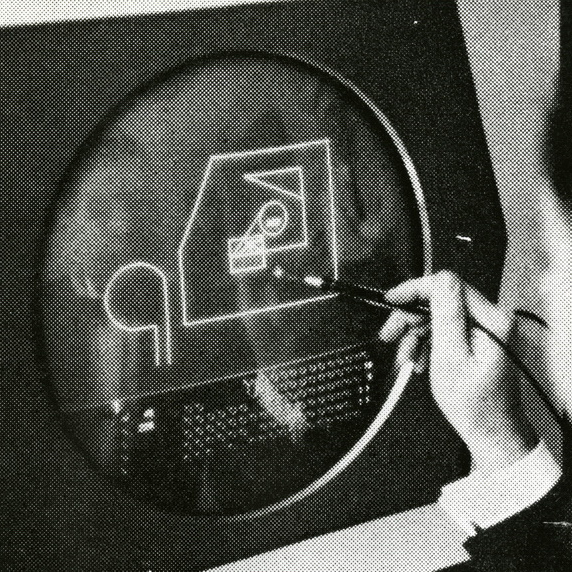
\includegraphics[width=8cm]{figuras/figura-1}}
		}{
			\Fonte{Elaborado pelo autor}
		}	
	\end{figure}
	
\lipsum[11]

\section{Trabalho Relacionado B}
\label{sec:trabalho-relacionado-b}

Integer non lacinia magna. Aenean tempor lorem tellus, non sodales nisl commodo ut. Proin mattis placerat risus sit amet laoreet. Praesent sapien arcu, maximus ac fringilla efficitur, vulputate faucibus sem. Donec aliquet velit eros, sit amet elementum dolor pharetra eget. Integer eget mattis libero. Praesent ex velit, pulvinar at massa vel, fermentum dictum mauris. Ut feugiat accumsan augue, et ultrices ipsum euismod vitae

	\begin{figure}[h!]
		\centering
		\Caption{\label{fig:exemplo-2} Maecenas luctus augue odio, sed tincidunt nunc posuere nec}	
		\UNIFORfig{}{
			\fbox{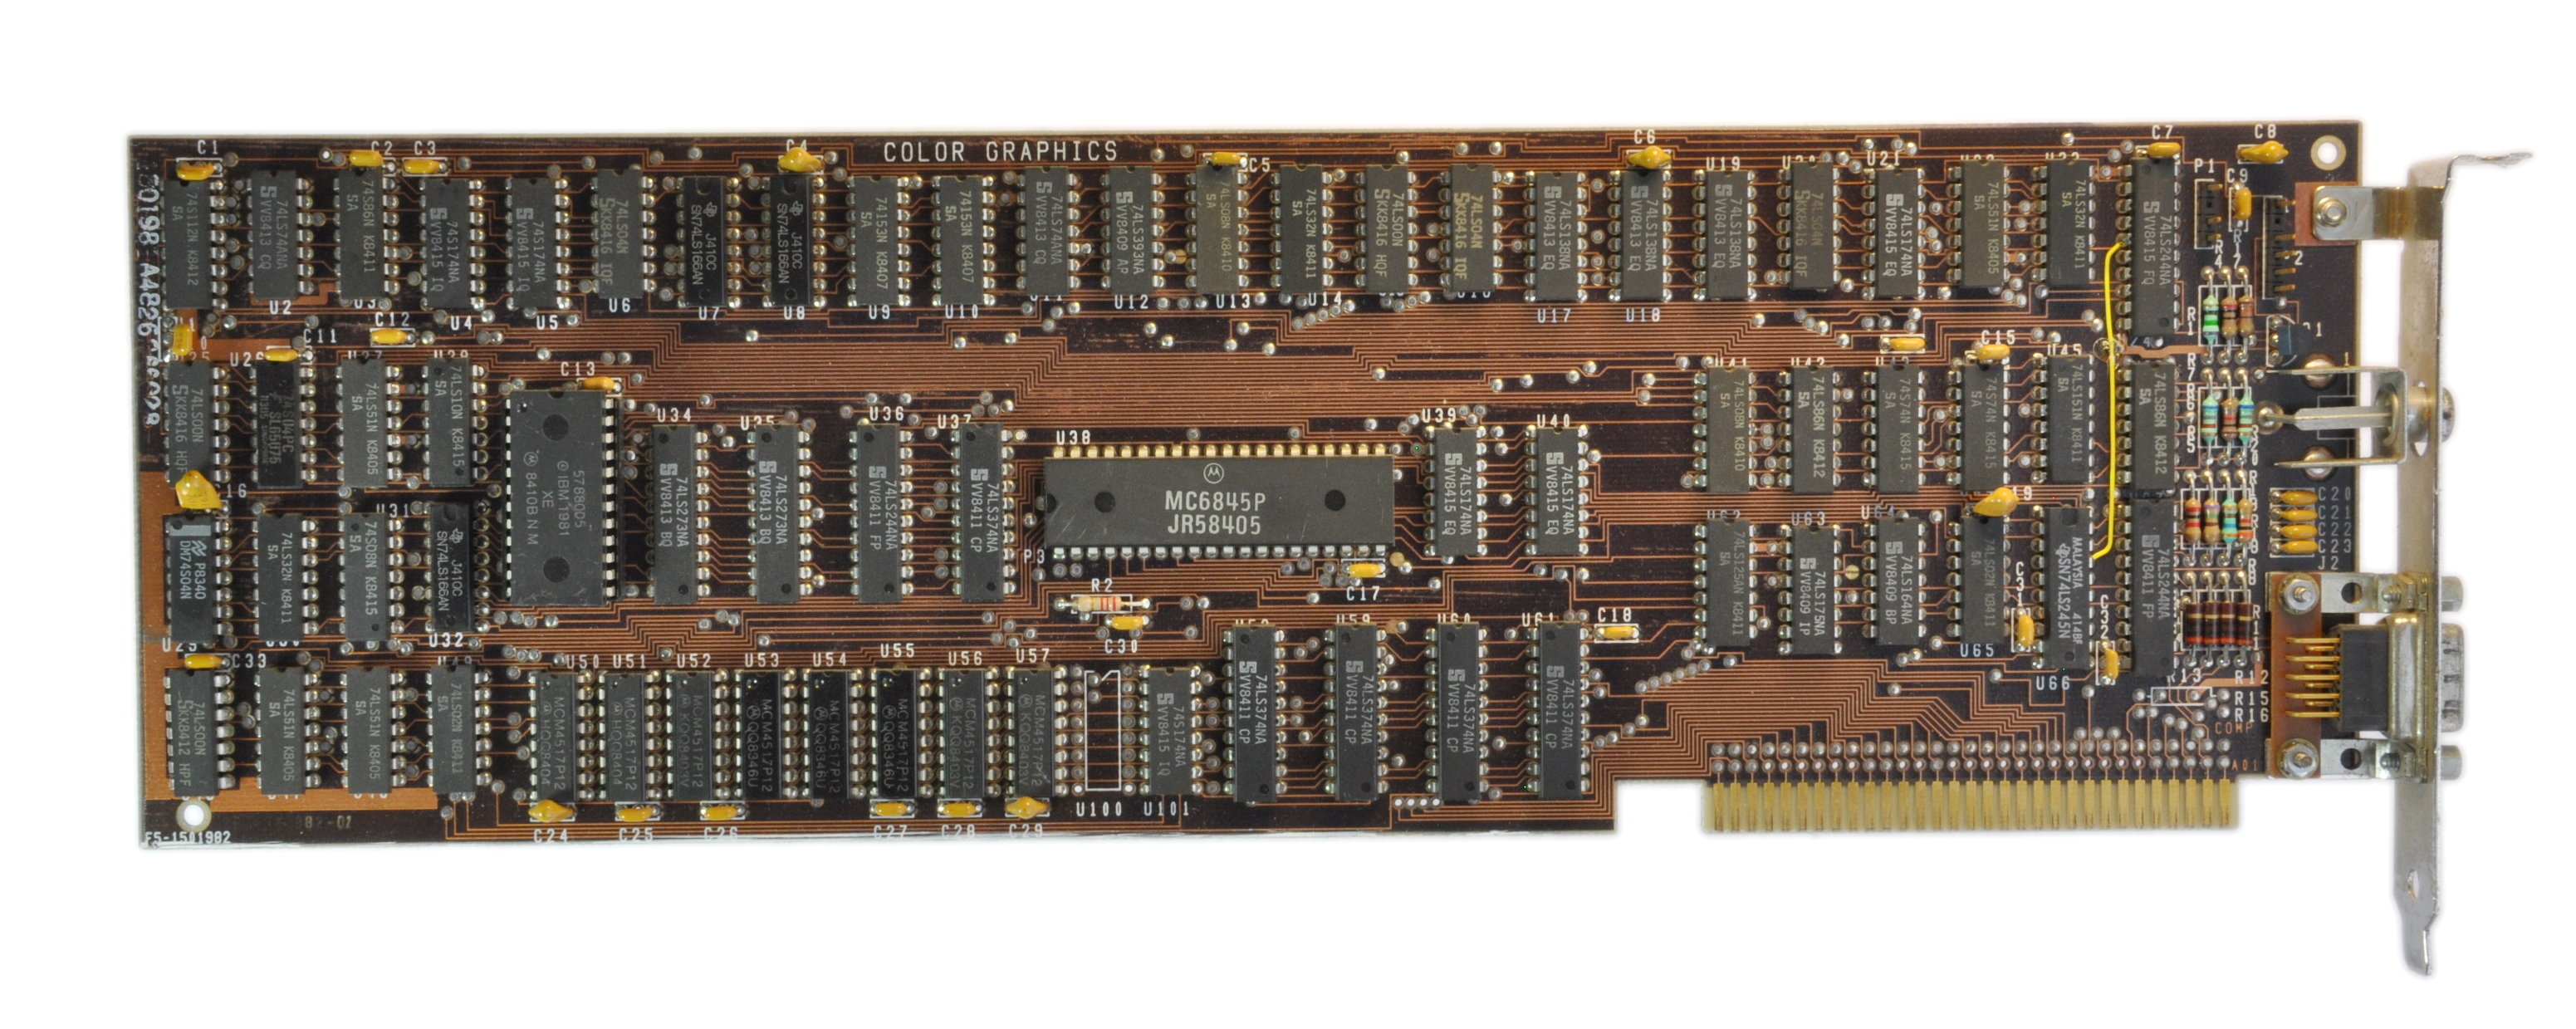
\includegraphics[width=8cm]{figuras/figura-2}}
		}{
			\Fonte{Elaborado pelo autor}			
		}	
	\end{figure}

Nunc ac pretium dui. Mauris aliquam dapibus nulla ac mattis. Aenean non tortor volutpat, varius lectus vitae, accumsan nibh. Cras pretium vestibulum enim, id ullamcorper tortor ultrices non. Integer sodales viverra faucibus. Curabitur at dui lacinia, rhoncus lacus at, blandit metus. Integer scelerisque non enim quis ornare.

	\begin{quadro}[h!]	
		\centering
		\Caption{\label{qua:exemplo-1} Praesent ex velit, pulvinar at massa vel, fermentum dictum mauris. Ut feugiat accumsan augue}		
		\UNIFORqua{}{
			\begin{tabular}{|c|c|l|l|}
				\hline
				Quisque & pharetra & tempus & vulputate \\
				\hline
				E1 & Complete coverage by a single transcript & Both  & Complete\\
				\hline
				E2 & Complete coverage by more than & Both splice sites & Complete\\
				\hline
				E3 & Partial coverage & Both splice sites & Both \\				
				\hline
			\end{tabular}
		}{
			\Fonte{Elaborado pelo autor}
		}
	\end{quadro}
	
\lipsum[20]

	
	\begin{quadro}[h!]	
		\centering
		\Caption{\label{qua:exemplo-2} Duis faucibus, enim quis tincidunt pellentesque}		
		\UNIFORqua{}{
			\begin{tabular}{|c|c|}
				\hline
				Quisque & pharetra \\
				\hline
				E1 & Complete coverage by a single transcript \\
				\hline
				E2 & Complete coverage by more than \\
				\hline
				E3 & Partial coverage \\
				\hline
				E4 & Partial coverage \\
				\hline
				E5 & Partial coverage \\
				\hline
				E6 & Partial coverage \\
				\hline
				E7 & Partial coverage \\
				\hline
			\end{tabular}
		}{
			\Fonte{Elaborado pelo autor}
		}
	\end{quadro}

\lipsum[21]

Integer non lacinia magna. Aenean tempor lorem tellus, non sodales nisl commodo ut. Proin mattis placerat risus sit amet laoreet. Praesent sapien arcu, maximus ac fringilla efficitur, vulputate faucibus sem. Donec aliquet velit eros, sit amet elementum dolor pharetra eget. Integer eget mattis libero.
\Gls{ambiguidade}
\Gls{braile}
\Gls{coerencia}
\Gls{dialetos}
\Gls{elipse}
\Gls{locucao-adjetiva}
\Gls{modificadores}
\Gls{paronimos}
\Gls{sintese}
\Gls{borboleta}
	\chapter{Metodologia}
\label{chap:metodologia}

\lipsum[2]
\lipsum[12]

O autor \lipsum[2] 

\begin{table}[h!]
	\Caption{\label{tabela-ibge} Um Exemplo de tabela alinhada que pode ser longa ou curta, conforme padrão IBGE}%
	\IBGEtab{}{%
		\begin{tabular}{ccc}
			\toprule
			Nome & Nascimento & Documento \\
			\midrule \midrule
			Maria da Silva & 11/11/1111 & 111.111.111-11 \\
			Maria da Silva & 11/11/1111 & 111.111.111-11 \\
			Maria da Silva & 11/11/1111 & 111.111.111-11 \\
			\bottomrule
		\end{tabular}%
	}{%
	\Fonte{Produzido pelos autores}%
	\Nota{Esta é uma nota, que diz que os dados são baseados na
		regressão linear.}%
	\Nota[Anotações]{Uma anotação adicional, seguida de várias outras.}%
}
\end{table}

 \lipsum[2] 

\section{Exemplo de Algoritmos e Figuras}
\label{sec:exemplo-de-algoritmos-e-figuras}

\lipsum[2]

\begin{algorithm}[h!]
	\SetSpacedAlgorithm
	\caption{\label{exemplo-de-algoritmo}Como escrever algoritmos no \LaTeX2e}
	\Entrada{o proprio texto}
	\Saida{como escrever algoritmos com \LaTeX2e }
	\Inicio{
		inicializa\c{c}\~ao\;
		\Repita{fim do texto}{
			leia o atual\;
			\Se{entendeu}{
				vá para o próximo\;
				próximo se torna o atual\;}
			\Senao{volte ao início da seção\;}
		}
	}	
\end{algorithm}

\lipsum[2]
%\begin{algorithm}[H]
%	\Entrada{o proprio texto}
%	\Saida{como escrever algoritmos com \LaTeX2e }
%	\Inicio{
%		inicializa\c{c}\~ao\;
%		\Repita{fim do texto}{
%			leia o atual\;
%			\Se{entendeu}{
%				vá para o próximo\;
%				próximo se torna o atual\;}
%			\Senao{volte ao início da seção\;}
%		}
%	}
%	\caption{Exemplo de Algoritmo Versao 02}
%\end{algorithm}

%\begin{algorithm}
%	\begin{algorithmic}
%	\Entrada{o proprio texto}
%	\Saida{como escrever algoritmos com \LaTeX2e }	
%	\end{algorithmic}
%\end{algorithm}

Exemplo de alíneas com números:

\begin{alineascomnumero}
	\item Lorem ipsum dolor sit amet, consectetur adipiscing elit. Nunc dictum sed tortor nec viverra.
	\item Praesent vitae nulla varius, pulvinar quam at, dapibus nisi. Aenean in commodo tellus. Mauris molestie est sed justo malesuada, quis feugiat tellus venenatis.
	\item Praesent quis erat eleifend, lacinia turpis in, tristique tellus. Nunc dictum sed tortor nec viverra.
	\item Mauris facilisis odio eu ornare tempor. Nunc dictum sed tortor nec viverra.
	\item Curabitur convallis odio at eros consequat pretium.
\end{alineascomnumero}

\lipsum[12]

\begin{table}[h!]	
	\centering
	\Caption{\label{tab:internal}Internal exon scores}	
	\IBGEtab{}{
		\begin{tabular}{cll}
			\toprule
			Ranking & Exon Coverage & Splice Site Support\\
			\midrule \midrule
			E1 & Complete coverage by a single transcript & Both splice sites\\
			E2 & Complete coverage by more than a single transcript & Both splice sites\\
			E3 & Partial coverage & Both splice sites\\
			E4 & Partial coverage & One splice site\\
			E5 & Complete or partial coverage & No splice sites\\
			E6 & No coverage & No splice sites\\
			\bottomrule
		\end{tabular}
	}{
	\Fonte{os autores}
}
\end{table}

\lipsum[2] Referenciando a \autoref{tab:internal} \lipsum[2]

\index{figuras}Figuras podem ser criadas diretamente em LaTeX,
como o exemplo da \ref{fig-grafico-1}.

\begin{figure}[h!]
	\centering
	\Caption{\label{fig-grafico-1}Produção anual das dissertações de mestrado e teses de doutorado entre os anos de 1990 e 2008}		
	\IBGEtab{}{
		\fbox{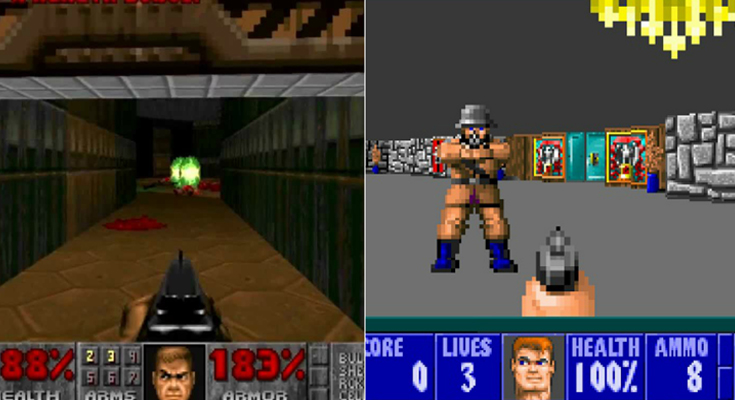
\includegraphics[scale=0.5]{figuras/figura-3}}
	}{
	\Fonte{os autores}
}
\end{figure}

Ou então figuras podem ser incorporadas de arquivos externos, como é o caso da \autoref{fig-grafico-1}. Se a figura que ser incluída se tratar de um diagrama, um gráfico ou uma ilustração que você mesmo produza, priorize o uso de imagens vetoriais no formato PDF. Com isso, o tamanho do arquivo final do trabalho será menor, e as imagens terão uma apresentação melhor, principalmente quando impressas, uma vez que imagens vetorias são perfeitamente escaláveis para qualquer dimensão. Nesse caso, se for utilizar o Microsoft Excel para produzir gráficos, ou o Microsoft Word para produzir ilustrações, exporte-os como PDF e os incorpore ao documento conforme o exemplo abaixo. No entanto, para manter a coerência no uso de software livre (já que você está usando LaTeX e abnTeX),  teste a ferramenta InkScape\index{InkScape}. ao CorelDraw\index{CorelDraw} ou ao Adobe Illustrator\index{Adobe! Illustrator}.  De todo modo, caso não seja possível  utilizar arquivos de imagens como PDF, utilize qualquer outro formato, como JPEG, GIF, BMP, etc.  Nesse caso, você pode tentar aprimorar as imagens incorporadas com o software livre \index{Gimp}Gimp. Ele é uma alternativa livre ao Adobe Photoshop\index{Adobe! Photoshop}.

\section{Usando Fórmulas Matemáticas}

\lipsum[2]

	\begin{equation}
		\begin{aligned}
			x = a_0 + \cfrac{1}{a_1
				+ \cfrac{1}{a_2
					+ \cfrac{1}{a_3 + \cfrac{1}{a_4} } } }
		\end{aligned}
	\end{equation}

\lipsum[3]

	\begin{equation}
		\begin{aligned}
			k_{n+1} = n^2 + k_n^2 - k_{n-1}
		\end{aligned}
	\end{equation}

\lipsum[4]

	\begin{equation}
		\begin{aligned}
			\cos (2\theta) = \cos^2 \theta - \sin^2 \theta
		\end{aligned}
	\end{equation}
	
\lipsum[5]

	\begin{equation}
		\begin{aligned}
			A_{m,n} =
			\begin{pmatrix}
			a_{1,1} & a_{1,2} & \cdots & a_{1,n} \\
			a_{2,1} & a_{2,2} & \cdots & a_{2,n} \\
			\vdots  & \vdots  & \ddots & \vdots  \\
			a_{m,1} & a_{m,2} & \cdots & a_{m,n}
			\end{pmatrix}
		\end{aligned}
	\end{equation}

\lipsum[6]

	\begin{equation}
		\begin{aligned}
			f(n) = \left\{ 
			\begin{array}{l l}
			n/2 & \quad \text{if $n$ is even}\\
			-(n+1)/2 & \quad \text{if $n$ is odd}
			\end{array} \right.
		\end{aligned}
	\end{equation}
	
\lipsum[7]

\section{Usando Algoritmos}

\lipsum[8]

\begin{algorithm}[h!]
	\SetSpacedAlgorithm
	\caption{\label{alg:algoritmo_de_colonica_de_formigas}Algoritmo de Otimização por Colônia de Formiga}
	\Entrada{Entrada do Algoritmo}
	\Saida{Saida do Algoritmo}
	\Inicio{
		Atribua os valores dos parâmetros\;
		Inicialize as trilhas de feromônios\;
		\Enqto{não atingir o critério de parada}{
			\Para{cada formiga}{
				Construa as Soluções\;
			}
			Aplique Busca Local (Opcional)\;
			Atualize o Feromônio\;
		}	
	}		
\end{algorithm}

\lipsum[9]

\section{Usando Código-fonte}

\lipsum[10]

\lstinputlisting[language=C++,caption={Hello World em C++}]{figuras/main.cpp}

\lipsum[11]

\begin{lstlisting}[language=Java,caption={Hello World em Java}]
public class HelloWorld {
	public static void main(String[] args) {
		System.out.println("Hello World!");
	}
}
\end{lstlisting}

\lipsum[11]

\section{Usando Teoremas, Proposições, etc}

Lorem ipsum dolor sit amet, consectetur adipiscing elit. Nunc dictum sed tortor nec viverra. consectetur adipiscing elit. Nunc dictum sed tortor nec viverra.

\begin{teo}[Pitágoras]
	Em todo triângulo retângulo o quadrado do comprimento da
	hipotenusa é igual a soma dos quadrados dos comprimentos dos catetos.
\end{teo}


Lorem ipsum dolor sit amet, consectetur adipiscing elit. Nunc dictum sed tortor nec viverra. consectetur adipiscing elit. Nunc dictum sed tortor nec viverra.

\begin{teo}[Fermat]
	Não existem inteiros $n > 2$, e $x, y, z$ tais que $x^n + y^n = z$
\end{teo}

Lorem ipsum dolor sit amet, consectetur adipiscing elit. Nunc dictum sed tortor nec viverra. consectetur adipiscing elit. Nunc dictum sed tortor nec viverra.

\begin{prop}
	Para demonstrar o Teorema de Pitágoras...
\end{prop}

Lorem ipsum dolor sit amet, consectetur adipiscing elit. Nunc dictum sed tortor nec viverra. consectetur adipiscing elit. Nunc dictum sed tortor nec viverra.

\begin{exem}
	Este é um exemplo do uso do ambiente exe definido acima.
\end{exem}

Lorem ipsum dolor sit amet, consectetur adipiscing elit. Nunc dictum sed tortor nec viverra. consectetur adipiscing elit. Nunc dictum sed tortor nec viverra.

\begin{xdefinicao}
	Definimos o produto de ...
\end{xdefinicao}

Lorem ipsum dolor sit amet, consectetur adipiscing elit. Nunc dictum sed tortor nec viverra. consectetur adipiscing elit. Nunc dictum sed tortor nec viverra.

\section{Usando Questões}


Lorem ipsum dolor sit amet, consectetur adipiscing elit. Nunc dictum sed tortor nec viverra. consectetur adipiscing elit. Nunc dictum sed tortor nec viverra.

\begin{questao}
	\item Esta é a primeira questão com alguns itens:
		\begin{enumerate}
			\item Este é o primeiro item
			\item Segundo item
		\end{enumerate}
	\item Esta é a segunda questão:
		\begin{enumerate}
			\item Este é o primeiro item
			\item Segundo item
		\end{enumerate}
	\item Lorem ipsum dolor sit amet, consectetur adipiscing elit. Nunc dictum sed tortor nec viverra. consectetur adipiscing elit. Nunc dictum sed tortor nec viverra.
		\begin{enumerate}
			\item consectetur
			\item adipiscing
			\item Nunc
			\item dictum
		\end{enumerate}
\end{questao}

\section{Citações}

\subsection{Documentos com três autores}

Quando houver três autores na citação, apresentam se os três, separados por ponto e vírgula, caso estes estejam após o texto. Se os autores estiverem incluídos no texto, devem ser separados por vírgula e pela conjunção "e".

%\citeautoronline{tresautores}


\subsection{Documentos com mais de três autores}
Havendo mais de três autores, indica-se o primeiro seguido da expressão \textit{et al.} (do latim \textit{et alli}, que significa e outros), do ano e da página.

%\citeautoronline{quatroautores}


\subsection{Documentos de vários autores}

Havendo    citações    indiretas de    diversos    documentos    de    vários    autores, mencionados  simultaneamente e  que  expressam  a  mesma  ideia,  separam-se  os  autores  por ponto e vírgula, em ordem alfabética.

\section{Notas de Rodap\'{e}}

Deve-se utilizar o sistema autor-data para as  citações no texto e o numérico para notas explicativas\footnote{Veja - se como exemplo desse tipo de abordagem o estudo de Netzer (1976)}. As notas de rodapé podem e devem ser alinhadas, a partir da segunda linha da mesma nota, abaixo da primeira letra da primeira palavra, de forma a destacar o expoente \footnote{Encontramos  esse  tipo  de  perspectiva  na  2ª  parte  do  verbete  referido  na  nota  anterior,  em  grande  parte  do estudo de Rahner (1962).} e sem espaço entre elas e com fonte menor (tamanho 10).


	\chapter{Resultados}
\label{chap:resultados}

A seguir são apresentados os resultados do estudo conduzido para cada um dos motores de jogo, aplicando as recomendações mencionadas na documentação de cada um e utilizando o cenário base de testes. Como cada motor utiliza o seu próprio formato de arquivo para manipular os \textit{assets}, para que fosse possível replicar o mesmo cenário nos três motores foi necessário utilizar um cenário pré-modelado, onde os objetos 3D foram posicionados fixamente.

\section{Discussão dos resultados na Unreal}
\label{sec:resultado-unreal}

Na Unreal, um ponto positivo vai para a existência de materiais de ambiente (Grama, tijolos, pedras e até água) já prontos para serem utilizados, e inclusive com otimizações de performance como nível de detalhe e tesselação, dentro da pasta de conteúdo inicial do template de projeto padrão. Isso ajuda a reduzir bastante o trabalho dos desenvolvedores ao implementar shaders em seus jogos.

A primeira recomendação na documentação da Unreal sugere desativar a projeção de sombra, que é uma opção que vem habilitada por padrão. As sombras fazem com que os objetos pareçam estar ancorados no mundo e dão ao observador uma sensação de profundidade e espaço. 

Sombras estáticas não são custosas no que diz respeito à renderização, mas sombras dinâmicas podem ser um dos maiores problemas de desempenho. Em média, as luzes de projeção de sombras dinâmicas móveis são as mais custosas (EPIC GAMES, 2021).

Para a realização desta etapa, foi desativa a projeção de sombra individualmente para cada malha e em seguida, com a projeção das malhas reativada, foi desativado apenas na fonte de luz direcional.

Por padrão, o Unreal Engine usa um renderizador diferido, pois ele fornece maior versatilidade e concede acesso a mais recursos de renderização. A renderização diferida não é apenas mais rápida, mas também oferece melhores opções de anti-aliasing, o que gera melhores aspectos visuais.

A renderização direta fornece uma linha de base com passagens de renderização mais rápidas. A segunda etapa então consistiu em mudar, nas configurações do projeto, o modo de renderização de diferido para direto.

A próxima etapa consistiu em ajustar a oclusão de HZB (\acrlong{HZB}) que tem um custo constante alto, mas um custo por objeto menor. A oclusão HZB funciona da mesma forma que a oclusão padrão, exceto que é mais conservadora na maneira que seleciona objetos, o que significa que menos objetos são eliminados como resultado (EPIC GAMES, 2021). 

Ele usa uma versão \textit{mipmap} do alvo de renderização de profundidade de cena para verificar os limites de um ator. Também requer menos buscas de textura ao amostrar de um \textit{mipmap} menos detalhado (EPIC GAMES, 2021)\nocite{unrealdocs}.

A aplicação de técnicas de otimização de performance na Unreal se mostra mais difícil por exigir um conhecimento da ferramenta de console da engine para aplicar comandos necessários para alterar aspectos que afetam a performance.

Um detalhe importante para levar em consideração é que ao invés de fornecer alternativas embutidas na própria engine, ela recomenda e oferece soluções de terceiros para realizar benchmark e otimizações de gráficos. Além disso, a sua documentação, diferente da Unity, não aborda tantas opções de melhorias de performance em um clique. 

Por isso ela é considerada um motor de jogo mais apropriado para usuários avançados, por entender que esses já possuem o conhecimento das técnicas necessárias para melhorar a performance e conseguem aplicá-las sem o auxilio de opções simples embutidas na engine.

A Tabela \ref{qua:unreal} mostra os resultados obtidos para a aplicação de cada etapa de otmização.

\begin{table}[h!]
	\Caption{\label{qua:unreal} Contagem de elementos presentes na cena de teste}\UNIFORqua{}{
	\begin{tabular}{|l|c|c|c|} \hline
		            & Vértices  & Triângulos & Qtd.  \\ \hline
		Casa        & 6901      & 4264       & 72    \\ \hline
		Plano       & 4         & 2          & 144   \\ \hline
		Árvores     & 794       & 368        & 288   \\ \hline
		Cercas      & 7156      & 3632       & 360   \\ \hline
		Cogumelos   & 2208      & 1056       & 360   \\ \hline
		Rochas      & ---       & ---        & ---   \\ \hline
		~Tipo 1     & 576       & 338        & 432   \\ \hline
		~Tipo 2     & 554       & 338        & 144   \\ \hline
		~Tipo 3     & 690       & 426        & 288   \\ \hline
		~Tipo 4     & 512       & 280        & 216   \\ \hline  
		~Tipo 5     & 120       & 62         & 72    \\ \hline
		Água        & 8         & 12         & 4     \\ \hline
		Soma        & 19523     & 10778      & 2380 \\ \hline
		Total       & 46464740  & 25651640   & ---   \\ \hline
	\end{tabular} 
	}{
		\Fonte{Elaborado pelo Autor (2021)}
	}
\end{table} 

TODO: DESCREVER OS RESULTADOS

\section{Discussão dos resultados na Unity}
\label{sec:resultado-unity}

Na Unity foi criado um novo projeto com template 3D. Em seguida foram importados os modelos dos objetos para compor a cena. Ao importar os objetos foram removidas as importações de materiais e animações, pois estes não serão utilizados. A cena final é composta por uma câmera com posição fixa e contém aproximadamente 3 milhões e 300 mil triângulos (5 milhões e 500 mil vértices) resultando em 7211 \textit{batches} (chamadas de desenho).

Para a criação dos materiais, foram utilizados os padrões da engine que consistem no shader de superfície padrão, exceto para a implementação de um shader de musgo que afeta as pedras e para o shader de água. Ambos foram escritos utilizando a linguagem \textit{ShaderLab} e constam nos Anexos \ref{an:codigo-fonte-musgo-unity} e \ref{an:codigo-fonte-agua-unity} respectivamente.

Por padrão, a Unity importa um rig genérico para modelos de não personagens. Isso faz com que um componente Animator seja adicionado se o modelo for instanciado no tempo de execução. Se o modelo não for animado por meio do sistema de animação, isso adiciona sobrecarga desnecessária ao sistema de animação, porque todos os animadores ativos devem ser marcados uma vez por quadro (UNITY TECHNOLOGIES, 2021)\nocite{unityTech2021}.

Desativar o rig em modelos não animados para evitar esta adição automática de um componente Animator e possível adição inadvertida de animadores indesejados a uma cena é uma boa prática para objetos não animados e foi utilizada nessa cena (UNITY TECHNOLOGIES, 2021). 

É importante ressaltar que ao criar um material na Unity ele já possui um shader padrão embutido, facilitando bastante a implementação de shaders básicos (como cores ou texturas). Ou seja, para implementar shaders simples não é necessário realizar nenhum tipo de programação.

Foram utilizadas as configurações pré-definidas da Unity (tamanho máximo de 2048x2048, compressão normal e algoritmo de redimensionamento Mitchell) para importação das texturas que compõem os materiais. A única mudança realizada foi a remoção do filtro bilinear.

As etapas de otimização seguem as recomendações descritas na documentação da Unity para melhorias de performance. A cada etapa foram medidas as estatísticas fornecidas pela engine para comparar os procedimentos.

A primeira etapa de otimização seguindo a recomendação da documentação da Unity consiste em utilizar tamanhos menores de textura. Para aplicações mobile, 2048x2048 ou 1024x1024 é um tamanho suficiente de atlas de textura, e 512x512 é um tamanho suficiente para texturas individuais aplicadas em modelos 3D. Em contrapartida isso pode gerar uma perda de qualidade visual.

A próxima etapa de otimização consiste em desabilitar o sinalizador de leitura e gravação dos modelos 3D, pois ele é habilitado por padrão para todos os modelos importados. A Unity exige que este sinalizador seja habilitado se um projeto estiver modificando uma malha em tempo de execução via \textit{script}, ou se a malha for usada como base para um componente MeshCollider (o que não é o caso nessa cena padrão). Se o modelo não for usado em um MeshCollider e não for manipulado por scripts, é recomendado desativar este sinalizador para salvar metade da memória do modelo.

Se o formato de compressão da textura selecionado não é adequado para a plataforma de destino, o Unity descompacta a textura quando ela é carregada, consumindo tempo de CPU e uma quantidade excessiva de memória. Esse é um problema mais comum em dispositivos Android, que geralmente oferecem suporte a formatos de compactação de textura amplamente diferentes, dependendo do chipset.

Mais uma etapa de otimização consiste em usar a compressão de malha quando for possível.  Habilitar a compactação de malha reduz o número de bits usados para representar os números de ponto flutuante para diferentes canais de dados de um modelo. Isso pode levar a uma pequena perda de precisão e os efeitos dessa imprecisão devem ser verificados pelos artistas antes do uso em um projeto final. É possível usar três diferentes níveis de compressão (Low, Medium, High).

Outra etapa recomendada pela Unity é o uso da funcionalidade \textit{Graphics jobs}, uma opção que determina se serão utilizadas \textit{worker threads} (são \textit{threads} que performam uma única tarefa, como \textit{culling} ou \textit{mesh skinning}). Em plataformas onde essa funcionalidade está disponível, ela pode melhorar consideravelmente a performance.

Uma técnica interessante consiste em reduzir a distância de projeção da câmera usando a propriedade \textit{Far Clip Plane}. Esta propriedade é a distância além da qual os objetos não são mais renderizados pela câmera. Para disfarçar o fato de que objetos distantes não são mais visíveis, é possível usar a névoa. Após reduzir a distância de 1000 para 77 foi possível obter o dobro de taxa de quadros (60 FPS).

Caso a névoa seja um aspecto indesejado no jogo, uma alternativa na próxima etapa consiste em ativar a oclusão para desativar a renderização de objetos que estão ocultos por outros objetos. A seleção de oclusão do Unity não é adequada para todas as cenas, pode levar a sobrecarga de CPU adicional e pode ser complexa para configurar, mas pode melhorar muito o desempenho em algumas cenas.

Focando na próxima etapa, é possível fazer uso da instanciação de GPU para desenhar (ou renderizar) várias cópias da mesma malha de uma vez, usando um número menor de chamadas. Isso é útil para desenhar objetos como edifícios, árvores, grama ou outras coisas que aparecem repetidamente em uma cena.

Esse é um método útil para renderizar malhas idênticas e cada instância pode ter parâmetros diferentes (por exemplo, cor ou escala) para adicionar variação e reduzir a aparência de repetição. Isso pode ainda reduzir o número de chamadas de desenho e melhorar significativamente o desempenho de renderização (UNITY TECHNOLOGIES, 2021)\nocite{unity2Tech2021}.

Há ainda uma etapa de definição do nível de cascatas de sombra. Basicamente, quanto mais cascatas forem utilizadas, menos as sombras são afetadas pelo \textit{aliasing} de perspectiva. Aumentar o número aumenta a sobrecarga de renderização. No entanto, essa sobrecarga ainda é menor do que seria no caso de um mapa de alta resolução em toda a sombra.

Outro processo descrito consiste em utilizar os shaders móveis otimizados embutidos na Unity; deve-se experimentar usá-los e ver se isso melhora o desempenho sem afetar a aparência do jogo. Esses shaders foram projetados para uso em plataformas móveis, mas são adequados para qualquer projeto. É perfeitamente normal usar shaders "móveis" em plataformas não móveis para aumentar o desempenho se eles fornecerem a fidelidade visual necessária para o projeto.

A Tabela \ref{qua:unity} mostra os resultados obtidos para a aplicação de cada etapa de otmização.

\begin{table}[h!]
	\Caption{\label{qua:unity} Dados estatísticos de renderização da Unity}\UNIFORqua{}{
	\begin{tabular}{|l|c|c|c|} \hline
		            & \makecell{\textit{Thread} \\ de renderização}  & \makecell{\textit{Batches} \\ (Salvo)} & FPS  \\ \hline
		Etapa 1 & & & \\ \hline
		~Textura 1024x1024 & 29.6 ms & 7211 (15342) & 28.1 \\ \hline
		~Textura 512x512 & 28.4 ms & 7211 (15342) & 28.9 \\ \hline
		Etapa 2 & & & \\ \hline
		~Sem Leitura e Escrita (Malha) & 26.5 ms & 7226 (15327) & 30.1 \\ \hline
		~Compressão baixa (Malha) & 28.7 ms & 7215 (15338) & 28.1 \\ \hline
		~Compressão média (Malha) & 31.6 ms & 7213 (15340) & 25.9 \\ \hline
		~Compressão alta (Malha) & 28.7 ms & 7199 (15354) & 28.6 \\ \hline
		Etapa 3 & & & \\ \hline
		~Graphic Job ativado & 29.2 ms & 7199 (15354) & 28.9 \\ \hline
		Etapa 4 & & & \\ \hline
		~Névoa ativada & 15.8 ms & 3397 (6778) & 56.7 \\ \hline
		~Culling ativado & 27.2 ms & 7199 (15354) & 29.8 \\ \hline
		~Instanciação de GPU & 14.7 ms & 2228 (20325) & 32.3 \\ \hline
		Etapa 5 & & & \\ \hline
		~Cascata de sombra (0) & 13.2 ms & 2056 (17783) & 41.4 \\ \hline
		~Cascata de sombra (2) & 14.2 ms & 2141 (18913) & 39.3 \\ \hline
		Etapa 6 & & & \\ \hline
		~Shaders \textit{mobile} & 28.1 ms & 7015 (15538) & 28.6 \\ \hline
	\end{tabular} 
	}{
		\Fonte{Elaborado pelo Autor (2021)}
	}
\end{table} 

TODO: DESCREVER OS RESULTADOS

	\chapter{Conclusão}
\label{chap:conclusao}

Tendo em vista os aspectos analisados nesse estudo, foi possível comparar as principais ferramentas de desenvolvimento de \textit{shaders} entre os motores de jogo Unity, Unreal e Godot com foco na otimização de performance em cada uma. 

Foi observado que a Unity mostrou-se como uma solução mais completa por oferecer, de maneira eficaz, ferramentas de análise de execução de \textit{shaders} e opções de otimização para o usuário. E também por disponibilizar \textit{shaders} otimizados para uso imediato. No final, mostrou-se como um motor de jogo mais amigável a novos usuários por conter uma documentação rica em detalhes e técnicas de otimização.

A Unreal também ofereceu uma variedade de \textit{shaders} otimizados (apesar de não serem voltados para dispositivos móveis), porém suas ferramentas de análise de desempenho e opções de otimização deixaram a desejar quando comparadas as da Unity. Sua documentação mostrou-se voltada para usuários com conhecimento avançado em técnicas de otimização. 

A Godot possui uma documentação muito boa, de leitura fácil, porém que peca por trazer exemplos muito generalizados de uso. Isso acabou por criar uma limitação de técnicas que poderiam ser aplicadas para otimizar os shaders. Além disso, os resultados obtidos com esse motor de jogo foram os piores dentre os três.

Uma recomendação interessante, que foi além do escopo desse estudo, consiste em desativar os \textit{mipmaps} para objetos que não apresentam grande variação de profundidade no campo de visão da câmera (como texturas com tamanho fixo), para salvar cerca de um terço de memória de carregamento de textura. Por outro lado, caso haja variação é recomendado ativar o uso de \textit{mipmaps} para melhorar a performance.

Cabe ressaltar que os objetos que compartilham configurações semelhantes podem ser combinados na mesma chamada de desenho através da criação de lotes. A CPU cria um pacote de dados para cada chamada. Às vezes, os lotes podem conter outros dados além das chamadas de desenho, mas é improvável que essas situações contribuam para problemas comuns de desempenho.

A CPU coleta informações sobre cada objeto que será renderizado e classifica esses dados em comandos conhecidos como chamadas de desenho. Uma chamada de desenho contém dados sobre uma única malha e como essa malha deve ser renderizada (por exemplo, quais texturas devem ser usadas). 

Outrossim, otimizar partes que não possuem relação com os gargalos é uma perda de tempo e provavelmente irá introduzir novos \textit{bugs} ou até mesmo regressões de desempenho em outros casos. A cada nova etapa de otimização, o ideal é utilizar a ferramenta de \textit{profiling} novamente, pois isso pode revelar um novo gargalo de desempenho que antes estava oculto.


	%Elementos pós-textuais
	\bibliography{elementos-pos-textuais/referencias}
	\imprimirglossario
	\imprimirapendices
		% Adicione aqui os apendices do seu trabalho
		\apendice{Coordenadas Homogêneas}
\label{ap:coordenadas-homogeneas}

As coordenadas homogêneas foram criadas para solucionar um problema presente na geometria do espaço Euclidiano, onde duas linhas paralelas no mesmo plano nunca poderão se cruzar. Isso só é interessante até o ponto em que precisamos definir o comportamento geometrico no espaço de projeção. Por exemplo na Figura \ref{fig:projecao} os trilhos se aproximam até que convergem no horizonte (um ponto no infinito no espaço Euclidiano) distante do observador (AHN, 2012)\nocite{homogenous}.

	\begin{figure}[h!]
		\centering
		\Caption{\label{fig:projecao} A ferrovia fica mais estreita e se cruza no horizonte.}
		\UNIFORfig{}{
			\fbox{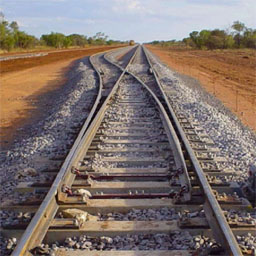
\includegraphics[width=8cm]{figuras/railroad}}
		}{
			\Fonte{\url{http://www.songho.ca/math/homogeneous/homogeneous.html}}
		}
	\end{figure}

Quando um ponto vai para o infinito ele é representado pelas coordenadas ($\infty$, $\infty$) e isso se torna uma informação inexpressiva. As linhas paralelas deveriam se cruzar no espaço de projeção mas não conseguem no espaço Euclidiano. Para resolver esse problema os matemáticos criaram as coordenadas homogêneas. O motivo de serem chamadas "homogêneas" se dá devido ao fato de que ao convertê-las para coordenadas cartesianas, percebe-se a relação de proporcionalidade explicitada na equação \ref{eq-homogenea5}, onde os diferentes pontos representam o mesmo ponto no espaço Euclidiano, ou seja, coordenadas homogêneas são invariantes à escala (AHN, 2012).

Coordenadas homogêneas são utilizadas para fazer a representação de coordenadas N-dimensionais utilizando N+1 números. Então para transformar um ponto de duas dimensões no sistema de coordenadas cartesianas (X, Y) basta simplesmente adicionar uma variável, portanto (x, y, w). A correlação matemática entre coordenadas cartesianas e coordenadas homogêneas é exibida abaixo na equação \ref{eq-homogenea}. Utilizando essa lógica fica claro que se um ponto (1, 2), se move em direção ao infinito, se tornando ($\infty$,$\infty$), ele passa a ser representado por (1, 2, 0) em coordenadas homogêneas, conforme a equação \ref{eq-homogenea2} (AHN, 2012).

\begin{equation} \label{eq-homogenea}
	\begin{aligned}
	X = \cfrac{x}{w} \\
	Y = \cfrac{y}{w} 
	\end{aligned}
\end{equation}

\begin{equation} \label{eq-homogenea2}
	\begin{aligned}
		(1,2,0) \rightarrow \left(\cfrac{1}{0}, \cfrac{2}{0}\right) \approx (\infty,\infty)
	\end{aligned}
\end{equation}

Para provar matematicamente que duas retas paralelas se cruzarão, basta analisar a equação \ref{eq-homogenea3} considerando a geometria Euclidiana. Nesse caso não há solução pois $ C \neq D $, apenas se as duas linhas fossem idênticas (sobrepostas) seria possível afirmar que $ C = D $. Para que o sistema possua solução é preciso reescrevê-lo como na equação \ref{eq-homogenea4}, trocando x e y por suas respectivas coordenadas homogêneas. Então como $ (C-D)w = 0 \therefore w=0 $, prova-se que as duas linhas paralelas são capazes de se cruzarem em (x, y, 0) que é um ponto no infinito (AHN, 2012).

\begin{equation} \label{eq-homogenea3}
	\begin{cases}
	Ax + By + C = 0 \\
	Ax + By + D = 0
	\end{cases}
\end{equation}

\begin{equation} \label{eq-homogenea4}
	\begin{cases}
	A\cfrac{x}{w} + B\cfrac{y}{w} + C = 0 \\
	A\cfrac{x}{w} + B\cfrac{y}{w} + D = 0
	\end{cases}
	\implies
	\begin{cases}
		Ax + By + Cw = 0 \\
		Ax + By + Dw = 0
	\end{cases}
\end{equation}

\begin{equation} \label{eq-homogenea5}
	\begin{split}
	(1,2,3) & \rightarrow \left(\cfrac{1}{3},\cfrac{2}{3}\right) \\
	(2,4,6) & \rightarrow \left(\cfrac{2}{6},\cfrac{4}{6}\right) = \left(\cfrac{1}{3},\cfrac{2}{3}\right) \\
	(4,8,12) & \rightarrow \left(\cfrac{4}{12},\cfrac{8}{12}\right) = \left(\cfrac{1}{3},\cfrac{2}{3}\right) \\
	\vdots \hspace{.8cm} & \rightarrow \hspace{.9cm} \vdots \\
	(1a,2a,3a) & \rightarrow \left(\cfrac{1a}{3a},\cfrac{2a}{3a}\right) = \left(\cfrac{1}{3},\cfrac{2}{3}\right)
	\end{split}
\end{equation}

		\apendice{Código-fonte do shader de contorno em HLSL}
\label{ap:codigo-fonte-contorno-hlsl}

\input{figuras/listings-glsl.prf}

	\begin{lstlisting}[language=GLSL, caption={\label{cf:outlineHLSL} Transcrição do shader de contorno de GLSL para HLSL}]
	Shader "Unlit/SimpleOutline" 
	{
		Properties 
		{
			_OutlineColor("Outline Color", Color) = (1,1,1,1)
			_OutlineWidth("Outline Width", Float) = 0.5
		}

		SubShader 
		{
			Tags {"Queue"="Transparent" "RenderType"="Opaque" }
			Cull Front
			Blend SrcAlpha OneMinusSrcAlpha

			Pass 
			{
				CGPROGRAM
				#pragma vertex vert
				#pragma fragment frag
				#include "UnityCG.cginc"

				struct appdata {
					float4 vertex : POSITION;
				};
				
				struct v2f {
					float4 vertex : SV_POSITION;
				};

				float4 _OutlineColor;
				float _OutlineWidth;

				v2f vert (appdata v) {
					v2f o;
					o.vertex = UnityObjectToClipPos(v.vertex);
					o.vertex.xyz *= _OutlineWidth;
					return o;
				}

				fixed4 frag (v2f i) : SV_Target {
					return _OutlineColor;
				}
				ENDCG
			}	
		}	
	}
	\end{lstlisting}

	\imprimiranexos
		% Adicione aqui os anexos do seu trabalho
		\anexo{Código-fonte do shader de contorno em GLSL}
\label{an:codigo-fonte-contorno-glsl}

\input{figuras/listings-glsl.prf}

\begin{lstlisting}[language=GLSL, caption={\label{cf:outline} Shader GLSL 3D simples para efeito de contorno}]
shader_type spatial;

render_mode unshaded, cull_front, depth_draw_always; 

uniform float thickness = 0.1; // espessura do contorno
uniform vec4 outline_color : hint_color = vec4(1.0); // cor do contorno

void vertex() {
    /* desloca cada vertice na direcao de sua normal vezes o fator de espessura */
	VERTEX += NORMAL * thickness; 
}

void fragment() {
    /* aplica a cor em cada pixel */
	ALBEDO = outline_color.rgb;
	if(outline_color.a < 1.0) ALPHA = outline_color.a;
}
\end{lstlisting}

\nocite{outlineGLSL}

\index{AAA}
	\imprimirindice

\end{document}
